\documentclass[
  11pt,
  twoside,
  a4paper,
  BCOR=8.25mm,
  parskip=half,
  numbers=noendperiod,
  toc=bib,
  chapterprefix=true]{scrbook}
\usepackage[utf8]{inputenc}
\usepackage[T1]{fontenc}
\usepackage{longtable}

\usepackage[square, numbers]{natbib}
\usepackage[titletoc]{appendix}
\RedeclareSectionCommand[tocbeforeskip=1ex plus 1pt minus 1pt]{chapter}

% \usepackage{libertineRoman}
\usepackage[bold]{roboto}
\usepackage[libertine,cmintegrals,cmbraces,vvarbb]{newtxmath}
\usepackage{mathpazo} % add possibly `sc` and `osf` options

% \renewcommand{\ttdefault{GoMono-TLF}}
\setkomafont{chapterentry}{\usefont{T1}{Crimson-TLF}{sb}{n}\large}

% \setkomafont{sectioning}{\usefont{T1}{Crimson-TLF}{m}{it}}
\setkomafont{chapter}{\usefont{T1}{PTSans-TLF}{m}{it}\fontsize{1.2cm}{1.5cm}\selectfont}
% \setkomafont{chapter}{\usefont{T1}{Crimson-TLF}{m}{it}\fontsize{1.2cm}{1.5cm}\selectfont}
\setkomafont{section}{\usefont{T1}{Crimson-TLF}{sb}{n}\LARGE}
\setkomafont{subsection}{\usefont{T1}{Crimson-TLF}{m}{it}\Large}
\setkomafont{subsubsection}{\usefont{T1}{Crimson-TLF}{m}{it}\large}
\setkomafont{paragraph}{\usefont{T1}{Crimson-TLF}{m}{it}\large}


\usepackage[scaled=0.9]{GoMono}
\usepackage[scale=0.93]{FiraSans}

\RedeclareSectionCommand[
  beforeskip=3em,
  afterskip=2em
]{chapter}

\RedeclareSectionCommand[
  % beforeskip=1em,
  beforeskip=0.9em,
  afterskip=0.4em
]{section}

\RedeclareSectionCommand[
  % beforeskip=1em,
  beforeskip=0.8em,
  afterskip=0.3em
]{subsection}

\RedeclareSectionCommand[
  % beforeskip=1em,
  beforeskip=0.4em,
  afterskip=0.3em
]{subsubsection}

% \RedeclareSectionCommand[
%   % beforeskip=1em,
%   beforeskip=0.5em,
%   afterskip=-0.8em
% ]{subsubsection}

\RedeclareSectionCommand[
  beforeskip=0em,
  % afterskip=0.05em
]{paragraph}

\RedeclareSectionCommand[
  beforeskip=0em,
  % afterskip=0.05em
]{subparagraph}

\renewcommand{\chapterheadmidvskip}{%
  \par\nobreak%\vskip -0.2em
}
\renewcommand*{\chapterformat}{%
  % \scalebox{2}{\sffamily \upshape \thechapter}%
  % \scalebox{1.5}{\sffamily \upshape \thechapter}%
  \fontsize{2.5cm}{1cm}\selectfont \upshape \roboto \color{black!40} \hfill \thechapter%
}
% \renewcommand{\raggedchapter}{\raggedleft}

% \renewcommand*{\sectionformat}{%
%   \makebox[0pt]{\makebox[2\linewidth][r]{\thesection}}%
% }

% \renewcommand*{\subsectionformat}{}
% \renewcommand*{\subsectionformat}{%
%   \makebox[0pt]{\makebox[2\linewidth][r]{\upshape\thesubsection}}%
% }

% \usepackage{placeins}

% \let\Oldsection\section
% \renewcommand{\section}{\FloatBarrier\Oldsection}

% \let\Oldsubsection\subsection
% \renewcommand{\subsection}{\FloatBarrier\Oldsubsection}

% \let\Oldsubsubsection\subsubsection
% \renewcommand{\subsubsection}{\FloatBarrier\Oldsubsubsection}

\usepackage{enumitem}
\setlist[description]{font=\rmfamily}

\usepackage[normalem]{ulem}
\renewcommand{\ULdepth}{1.8pt}
\makeatletter
\def\uwave{\bgroup \markoverwith{\lower3.5\p@\hbox{\sixly \textcolor{red}{\char58}}}\ULon}
\font\sixly=lasyb10 scaled 700 % does not re-load if already loaded, so no memory problem.
\makeatother

% To use graphics
\usepackage{graphicx}
\makeatletter
\def\maxwidth{\ifdim\Gin@nat@width>\linewidth\linewidth\else\Gin@nat@width\fi}
\def\maxheight{\ifdim\Gin@nat@height>\textheight\textheight\else\Gin@nat@height\fi}
\makeatother
\setkeys{Gin}{width=\maxwidth,height=\maxheight,keepaspectratio}

% For changing table sizes / columns
\usepackage{siunitx}
\usepackage{tabularx}
\usepackage{makecell}

% To force figures in place
\usepackage{float}

% Define thick column for tables
\makeatletter
\newcommand{\thickhline}{%
\noalign {\ifnum 0=`}\fi \hrule height 1.2pt
  \futurelet \reserved@a \@xhline
}
\makeatother
\newcolumntype{?}{!{\vrule width 1.2pt}}

\newcommand{\core}{{\color{ForestGreen} \small \sffamily \textbf{C}}}
\newcommand{\ext}{{\color{RedOrange} \small \sffamily \textbf{E}}}

% For hyperlinking inside the document
\usepackage[hidelinks,
  pdftitle={De-anonymizing encrypted video streams},
  pdfauthor={Stefano Peverelli}
]{hyperref}
\usepackage{cleveref}
\crefname{lstlisting}{listing}{listings}
\Crefname{lstlisting}{Listing}{Listings}
\Crefname{appsec}{Appendix}{Appendices}

% \def\sectionautorefname{Section}
% \def\sectionautorefname{Section}
% \def\subsectionautorefname{Subection}
% \newcommand*{\Appendixautorefname}{Appendix}

% To produce tightly spaced lists, used by pandoc
\providecommand{\tightlist}{%
  \setlength{\itemsep}{4pt}
  \setlength{\parskip}{0pt}
}

% Additional table options, allows to force it to \textwidth
\usepackage{tabularx}

% Provide \todo command to insert todo items in the document
\usepackage[dvipsnames]{xcolor,colortbl}
\newcommand{\todo}[1]{ {\color{RedOrange} \textit{\textbf{TODO:} #1}} }

% Make space befor "titled paragraphs" smaller
% \RedeclareSectionCommand[
  % beforeskip=.5\baselineskip]{paragraph}

% Remove numbers from sections
% \makeatletter
% \renewcommand{\@seccntformat}[1]{}
% \makeatother

% \makeatletter
% \def\@seccntformat#1{%
%   \expandafter\ifx\csname c@#1\endcsname\c@section\else
%   \csname the#1\endcsname\quad
%   \fi}
% \makeatother

% Only number sub-paragraphs
% \makeatletter
% \def\@seccntformat#1{%
%   \expandafter\ifx\csname c@#1\endcsname\c@subparagraph \thesubparagraph\enspace
%   \else
%   \fi}
% \makeatother

% Change sub-paragraph numbering format to only show one digit
% \renewcommand{\thesubparagraph}{\arabic{subparagraph}.}
% \renewcommand{\theparagraph}{\arabic{paragraph}.}
\setcounter{secnumdepth}{2}

\usepackage{listings}
\newcommand{\passthrough}[1]{#1}

\lstdefinelanguage{adu_lst}{
    morekeywords={
        ADU, SEQ, ID, GENRE, TITLE
    },
    sensitive=true,
    morecomment=[l]{//},
    morecomment=[l]{...},
    morecomment=[s]{/*}{*/},
    morestring=[b]"
}


\lstset{ 
  basicstyle=\footnotesize\ttfamily,        % the size of the fonts that are used for the code
  commentstyle=\itshape\color{gray},
  breakatwhitespace=true,         % sets if automatic breaks should only happen at whitespace
  breaklines=true,                 % sets automatic line breaking
  extendedchars=true,              % lets you use non-ASCII characters; for 8-bits encodings only, does not work with UTF-8
  %frame=single,	                   % adds a frame around the code
  keepspaces=true,                 % keeps spaces in text, useful for keeping indentation of code (possibly needs columns=flexible)
  keywordstyle=\bfseries,       % keyword style
  numbers=none,                    % where to put the line-numbers; possible values are (none, left, right)
  showspaces=false,                % show spaces everywhere adding particular underscores; it overrides 'showstringspaces'
  showstringspaces=false,          % underline spaces within strings only
  showtabs=false,                  % show tabs within strings adding particular underscores
  tabsize=2,	                   % sets default tabsize to 2 spaces
  xleftmargin=1.5em,
  belowskip=0pt,
  floatplacement={!htb},
  captionpos=b,
  moredelim={[is][\uwave]{__}{__}}
}

\lstdefinestyle{framedcode}{
  % float,
  floatplacement={!htbp},captionpos=b,
  frame=lines,xleftmargin=8pt,xrightmargin=8pt,
  %numbers=left,numberstyle=\footnotesize\ttfamily\color{gray},
  aboveskip=1.5em,
  xleftmargin=5pt,
  framexleftmargin=0pt,
}

\lstdefinestyle{snippet}{
  basicstyle=\ttfamily,keywordstyle=\color{blue},
  %backgroundcolor = \color{lightgray}
} 

\newenvironment{nsflalign*}
 {\setlength{\abovedisplayskip}{0pt}\setlength{\belowdisplayskip}{0pt}%
  \csname flalign*\endcsname}
 {\csname endflalign*\endcsname\ignorespacesafterend}

 \lstnewenvironment{adu}[1][]{%
    \lstset{language=adu_lst,style=framedcode,#1}}{}

 \lstnewenvironment{bash_script}[1][]{%
     \lstset{language=bash,style=snippet, #1}}{}

% \lstnewenvironment{sil}[1][]{%
%     \lstset{language=sil,
%         floatplacement={tbp},captionpos=b,
%         frame=lines,xleftmargin=8pt,xrightmargin=8pt,#1}}{}
% \newcommand{\silfile}[1]{
%   \lstinputlisting[language=sil,%
%     frame=lines,xleftmargin=8pt,xrightmargin=8pt,columns=fixed]{#1}
% }
% \def\inlinesil{%
%     \lstinline[language=sil,basicstyle=\ttfamily\small,columns=fixed]}

% \lstnewenvironment{code}[1][]%
% {
%    \noindent
%    \minipage{\linewidth}
%    \vspace{0.5\baselineskip}
%    \lstset{#1}}
% {\endminipage}

% \setlength{\abovecaptionskip}{0pt plus 2pt} % Chosen fairly arbitrarily

% \DeclareCaptionFormat{tabcap}{\small \textbf{#1#2}#3}
% \captionsetup[table]{format=tabcap}

% \captionsetup{format=bf-figcap,labelfont=bf}
\setkomafont{captionlabel}{\bfseries \small}
\setkomafont{caption}{\small}

\usepackage{caption}
\usepackage{subcaption}
\usepackage{multirow}
\usepackage{multicol}
\usepackage{rotating}

\usepackage{layout}
\usepackage{geometry}

\usepackage{pdfpages}

% To fix some boxes going over the margins (e.g. inline code)
\setlength\emergencystretch{\hsize}

\makeatletter
\captionsetup{margin=1em,
              labelsep=colon,
              format=hang,
              indention=-3em,
              parskip=5pt}
\newcommand{\Melissa[1]}{}

\AtBeginDocument{%
\renewcommand*\figurename{Figure}
\renewcommand*\tablename{Table}
}
\AtBeginDocument{%
\renewcommand*\listfigurename{List of Figures}
\renewcommand*\listtablename{List of Tables}
}
\makeatother

\begin{document}

\newgeometry{margin=1.5in}
\begin{titlepage}
  \centering \itshape
  \vspace*{6em}{
    {\Huge De-anonymizing \\ Encrypted Video Streams\par}
  }

  \vspace*{1em}{\Large Master's Thesis}\par
  14 September 2019\par

  \vspace*{4em}{\huge Stefano Peverelli \\
  \small \upshape \url{pstefano@student.ethz.ch}}\par

  \vspace*{2em}{\large supervised by \\
  \Large \itshape Prof. Dr. Ankit Singla
  \Large \itshape \&
  \Large \itshape Melissa Licciardello}

  \vspace*{20em}{
  \normalsize \upshape Systems Group\\
  Department of Computer Science\\
  ETH Zürich}

\end{titlepage}
\restoregeometry

\addchap*{\centering Abstract}

In recent years, tools for program verification have made significant progress
and are becoming more widely used. Yet, they still lack effective facilities to
allow investigating and understanding verification errors, especially when the
input program makes use of more advanced language features, such as quantified
permissions in Viper.

We think the most effective way to help a user in identifying the source of
a verification error is by employing a visual debugging approach, therefore we
want to provide a technique to automatically produce small, visual
counterexamples based on the information provided by a symbolic execution
engine.

We conducted a feasibility study to understand whether we could effectively
generate counterexamples via bounded modeling with Alloy, a language and
analyser for software modeling. The main idea behind this methodology is that
Alloy, because it performs a bounded search, is not affected by the problems
involving quantifier instantiation, and is therefore able to provide complete
concrete models in situations where the SMT solver would not.

In our technique, we encode the information about a symbolic execution state
into a model and use Alloy to generate instances of it. These instances
can then be used to build a visual diagram of the program's state. When the
state being modeled is one where a verification error occurred, and we
additionally encode the last failed query performed to the SMT solver, then the
instances Alloy generates are counterexamples to the failed verification.

As part of our feasibility study, we have implemented a subset of the technique
described in this thesis into a tool, integrated with the Viper IDE. This proof
of concept for a debugger demonstrates that our approach for visualizing
counterexamples to verification failures in the context of symbolic execution is
a feasible one and is worth exploring in more detail.


{
\setcounter{tocdepth}{2}
\tableofcontents
}

\chapter{Introduction}\label{sec:introduction}

According to the latest Cisco's VNI \cite{video-traffic-forecast}, video will
account for 82\% of all IP traffic in Europe by 2021; in addition, the overall IP
traffic per person will triplicate from 13\emph{GB} to 35\emph{GB}. These
forecasts clearly picture the growth of the streaming industry, posing, at the
same time an important question on the present and future states of the final
user's privacy.

As shown by Reed et Al. \cite{netflix-real-time} anonimity of user's viewing
activity is at risk. Not for the use that Netflix or other streaming services
do of user's session data, but because of the risk of a man-in-the-middle
attack, \emph{MITM}, carried by an \textit{evil} party that has control over the
flow of packets over a network.

In particular, they have shown how the adoption of HTTPS to protect video
streams from Netflix \emph{CDN}s to user's end devices, does not hold against
passive traffic analysis.

\section{Motivation}\label{motivation}

The goal of this project is to replicate part of the work conducted by Reed et
Al. and to investigate the possibility of identifying a Netflix stream solely
based on the observed average bandwidth. 

Specifically, we have built a system capable of manipulating network bandwidth,
observe video traffic, and reconstruct a \emph{bitrate ladder} for each video
being watched. We then build a library of fingerpints at various network
bandwidths, and analyze how often videos can be identified successfully, and
how many bitrate ladders are unique.

This, follows from the intuition that \emph{per-title encoding} embeds the
nature and the complexity of video frames in a unique way, that may reveal the
identity of the content being streamed.

Furthermore we investigate and discuss possible countermeasures that streaming
providers could adopt to preserve users privacy. A detailed explanation of our
approach is presented in \Cref{sec:approach}

\subsection{Per-Title Encoding}\label{sec:per-title-encoding}

In December 2015 Netflix announced \cite{per-title-encoding} that it was
introducing a new method to analyze the complexity of each title, and find the
best encoding recipe based on it. Their goal with the adoption of
per-title encoding was to provide users with better quality streams at a lower
bandwidth. 

Before then, each title was encoded with a \emph{Fixed Bitrate Ladder}; their
pipeline returned a list of \{\emph{Bitrate, Resolution}\} pairs that
represented the sufficient bitrate to encode the stream at a certain
resolution (\Cref{tab:fixed-ladder}), with no visible artificats.

\begin{table}[htb]
  \centering
  \begin{tabular}{|c|c|}
    \hline
    \textbf{Bitrate (kbps)} & \textbf{Resolution} \\
    \hline
    235                     &    $320\times240$ \\
    \hline
    375                     &    $384\times288$ \\
    \hline
    560                     &    $512\times384$ \\
    \hline
    750                     &    $512\times384$ \\
    \hline
    1050                    &    $640\times480$ \\
    \hline
    1750                    &    $720\times480$ \\
    \hline
    2350                    &   $1280\times720$ \\
    \hline
    3000                    &   $1280\times720$ \\
    \hline
    4300                    &   $1920\times1080$ \\
    \hline
    5800                    &   $1920\times1080$ \\
    \hline
  \end{tabular}
  \caption{Netflix original's Fixed Bitrate Ladder.}
  %\end{center}
  \label{tab:fixed-ladder}
\end{table}

This "one-size-fits-all" ladder, as reported, achieved good results in the
encoded video's perceived quality (\textbf{PSNR} \cite{psnr}) given the bitrate
constraint, but, would not perform optimally under certain conditions. For
instance, high detailed scenes with sudden changes of light, or rapid
transitions of camera shots, would require more than 5800\emph{kbps}; in
contrast, more static frames, as in animated cartoons, may be encoded at higher
resolutions mantaining the same bitrate level.

In summary they noticed how in certain cases, the produced encoding would
either present some small artifacts (\emph{e.g.} complex scenes), or waste
bandwidth, (\emph{e.g.} static, plain scenes). For this reason, they came up
with per-title encoding.

\begin{table}[htb]
  %\begin{center}
  \centering
  \begin{tabular}{|c|c|c|}
    \hline
    \textbf{Resolutions} & \textbf{Fixed Bitrate Ladder (kpbs)} & \textbf{Per-Title Bitrate Ladder (kbps)} \\
    \hline
    $320\times240$       & 235                                  & 150 \\
    \hline
    $384\times288$       & 375                                  & 200 \\
    \hline
    $512\times384$       & 560                                  & 290 \\
    \hline
    $512\times384$       & 750                                  & \\
    \hline
    $640\times480$       & 1050                                 & \\
    \hline
    $720\times480$       & 1750                                 & 440\\
    \hline
    $720\times480$       &                                      & 590\\
    \hline
    $1280\times720$      & 2350                                 & 830\\
    \hline
    $1920\times1080$     & 3000                                 & 1150\\
    \hline
    $1920\times1080$     & 4300                                 & 1470\\
    \hline
    $1920\times1080$     & 5800                                 & 2150\\
    \hline
    $1920\times1080$     &                                      & 3840\\
    \hline
  \end{tabular}
  \caption{
    Comparison between the two different approaches for the same title: note
    how different titles may have different numbers of quality levels. For each
    movie, the minimum number of quality levels gets computed to produce a
    just-noticeable-difference (JND), when switching bitrates during playback.
  }
  \label{tab:old-vs-new-ladder}
\end{table}

In order to find the best fitting bitrate ladder for a particular title, there
are several criterias that they took into account, the principal ones being:

\begin{itemize}
    \item How many quality levels should be encoded to obtain a
          \emph{JND} between each of them.
    \item Best \{\emph{Resolution, Bitrate}\} pair for each quality level
    \item Highest bitrate required to achieve the best perceivable quality
\end{itemize}

As aforementioned, each title's perceived video quality, gets computed as a
measure of \emph{Peak signal-to-noise ratio}. The comparison is performed
between the produced encode, upsampled to 1080\emph{p}, and the original title
in 1080\emph{p}, and the best \{\emph{Bitrate, Resolution}\} pair is assigned
to that specific quality level, as depicted in \Cref{tab:old-vs-new-ladder}.

In \Cref{fig:new-vs-old-ladder}, we can see the impact of per-title encoding on
the original bitrate ladder: in order to achieve the same perceivable quality
level (point \textbf{B} and \textbf{C}), it requires a lower bitrate to be
encoded to (point \textbf{A}).  Moreover, with around the same bitrate, one can
see how per-title encoding can achieve a higher resolution compared the fixed
case (point \textbf{A} and \textbf{D} respectively). It follows obviously that,
holding to a high-quality stream while maintainig or lowering the used
bandwidth is key: the end user will get same or better quality then before, at
a lower bandwidth.

\begin{figure}[!htb]
  \centering
  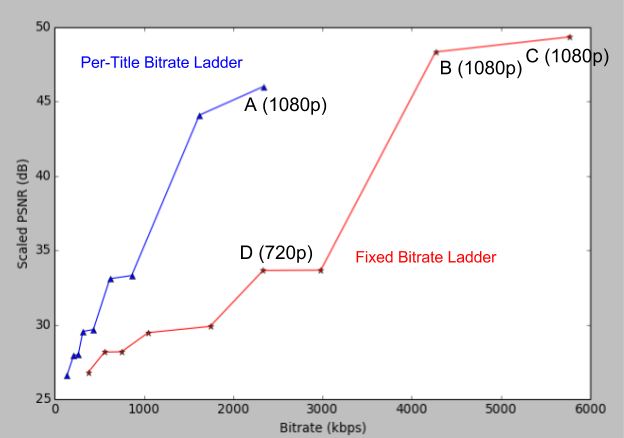
\includegraphics[width=0.9\columnwidth]{img/pertitlevsfixed.png}
  \caption{Difference between per-title vs. fixed bitrate ladders.}
  \label{fig:new-vs-old-ladder}
\end{figure}

\subsection{User's Privacy}\label{sec:privacy}

As of 2018, data began the most valuable commodity on the planet
\cite{data-value}, and with its value rising, society starts to question how to
legislate to protect both industry's and user's rights.

In 2016, Netflix announced the introduction of HTTPS to protect the content
being streamed to users. With the addition of TLS on top of HTTP, Netflix aim,
was to avoid the risk of eavesdropping on unsecure connections, protecting
themselves and users, from third-party applications and governments potentially
collecting viewer's data and streaming habits.

Avoiding deep packet inspection from potential eavesdropper certainly adds
another layer of security, but given the narrow relationship between Netflix
and ISPs, one might conclude that the chance that IP packets do not get
inspected by ISPs (especially in the United States, after the reclassification
of ISPs as Title I \emph{Information Services} \cite{net-neutrality}), is still
a matter of mere trust given to the platform-provider relationship.

Cases of user's data breaches as the Kanopy one \cite{kanopy}, are a testimony
of how easy would be for an attacker to extract information to the point at
which users could become identifiable by the solely information the platform
was collecting in their internal log files. The content of which, include
between others: timestamps, geo-location data, client-device informations and
IP addresses. 

The ability to cluster people based on just their video-streaming habits, poses
a potential threat for how the data could be processed and used by parties with
access to it. One could imagine how government agencies could easily get in
possession of sensitive information about the nature of the content a
particular user is interested about, or how ISPs could profit from selling data
profiles to advertisement companies, that in turn, would exploit their
information to improve per-user recommendation algorithms.

Considering this trend, it is for us crucial to investigate how parties that
can have access to transport-layer information, (more details in
\Cref{sec:approach}), could exploit per-title encoding to identify video
traffic. 

\section{Related Work}\label{related}

As previously mentioned, our work is mainly insipired by Reed et Al.'s
\cite{netflix-real-time} research paper, in which they presented a novel method
to de-anonymize encrypted netflix stream in real-time with limited hardware
requirements. Their system was able to identify a video using uniquely TCP/IP
headers, by making use of \texttt{adudump}, a command-line program built on top
of \emph{libpcap} \cite{libpcap}, a powerful C library for network traffic
capture. They acquired for each video, metadata information with a tampering
tool, and then matched adudump traces against with. The evaluation of their
method revelaed that they could identify majority of videos by recording only
20 minutes of traffic each. 

An earlier proof on how bandwidth analysis could reveal the content of
ecnrypted traffic, was given by Saponas et Al. \cite{Saponas2007devices}, in
their "SlingBox-Pro" case study, they investigate how a device that allowed
users to remotely stream the contents of their TV over the Internet, could leak
information on the video-content due to variabe bitrate encoding. They acquired
traces of the same content at different network bandwidth levels, and combined
into a database for future use. Then they presented a novel method that showed
how with a Discrete Fourier Transform based matching algorithm they could query
the aforementioned database. By analyzing 10 minutes of video they could
identify a video with 62\% of probability, and with 40 minutes, more than 77\%.

Other work that exploits VBR leakage has been done by Liu et Al.
\cite{forensic}.  In their model they try to overcome some of the typical
limitations of performing traffic analysis on video streams such as: a time
consuming attack process, the fact that network conditions regarding each
experiment are nearly identical (while in practice this depends on end-to-end
network stability), and the fact that usually the size of video streams is
limited to a pre-known set, and eventually that the performance of the
underlying model on a larger database remains unknown. They have introduced a
wavelet-based method to extract long and short range dependencies on the
recorded video traffic traces, achieving an accuracy of 90\% with only 3
minutes of video capture, and only a 1\% false alarm rate.

Another machine learning based approach, \cite{qoe}, addresses the problem
of estimating the QoE \emph{Quality of Experience} of video stream traffic.
Adudump is used to get a reconstruction of the video segment sizes, and then
some KPI \emph{Key Performance Indicator}, such as the initial video delay,
stalls due to low download rates, and average representation quality (average
throughput), are computed. Subsequently each video gets assigned a quality
level, and the collected features are trained with several classification
models (Naive Bayes, Random forests, SMOs). They are able to assess with 80\%
of accuracy the quality level of a video traffic trace recorded at an unseen
network bandwidth. 

Similar work has been conducted also by Moser \cite{moser}, who analyzed how
bitrate ladders could uniquely embed the identity of Netflix titles. In his
work he further studies the impact of the aggregation of each video's segment
bandwidth on the overall accuracy of his system. 

Note how in our approach, contrary to Moser's and Reed et Al's scenarios after
a recent Netflix update to its video player, it is no longer possible to force
the playback of a movie by simply choosing a certain quality level. This makes
the process of creating video fingerprints more challenging as we descirbe
throghout the rest of this document.

In addition, in Reed et Al's work, there is no evidence of TCM multiplexing.
This is verified by looking at their network capture traces \cite{traces}.
In \Cref{sec:results} we show how and in which scenarios, this affects our
measurements.

\section{Structure of this Report}\label{sec:structure}
  
In this section, we outline the contents and the structure of this report.

\Cref{sec:introduction} introduced our motivation behind the project, presented featured work
that influenced and inspire our approach, and listed the goals we would like to
ultimately achieve.

\Cref{sec:attack_isp} presents the attack scenario from the perspective of a
malicious user that has compromised a node on the path between the client and
the server, the infrastructure needed to acquire the data, the nature of the
information that could be infered, and the consequences that might arise.

\Cref{sec:approach} shows our version of the attack, in a different context, but up to
some extent, with similar conditions to the one depicted in Chapter 2. It also
higlights the similiarities and differences from the featured approaches we
followed.

\Cref{sec:results} we evaluate our system, we present results, and discuss the
relevance of such a method.

\Cref{sec:conclusion} tries to summarize and draw conclusions based on the claims made at
the beginning of this report.
%TODO Chapter 2 - End to End Attack Scenario 
               %- Describe the attack scenario from the perspective of an ISP
               %- Describe the infrastructure
               %- Describe what kind of information the attacker is able to retrieve
               %- Outline the consequences of such an attack
%TODO Chapter 3 - Approach
               %- Present our version of the attack scenario
               %- Describe the infrastructure
               %- Present the data we have collected
               %- Highlight the differences from our approach to Reed's et Al.
               %- Explain how we can uniquely identify a movie / Explain how we
                  %make use of the features we collect
%TODO Chapter 4 - Evaluation of the system
               %- Explain Plots & result data
%TODO Chapter 5 - Conclusion
               %- Future Work
               %- Acknowlegments

\chapter{ISPs as adversaries}\label{sec:attack_isp}

Of great importance to our approach, is aquiring real-time network traffic,
with downstream throughput being our only focus; here we discuss the potential
scenarios that allow adversaries to obtain such information, and describe how,
in particular ISPs, could make use of it, to identify video streaming and
profile users based on their streaming habits.

\section{Netflix-ISP relationship}

\begin{figure}[!htb]
  \centering
  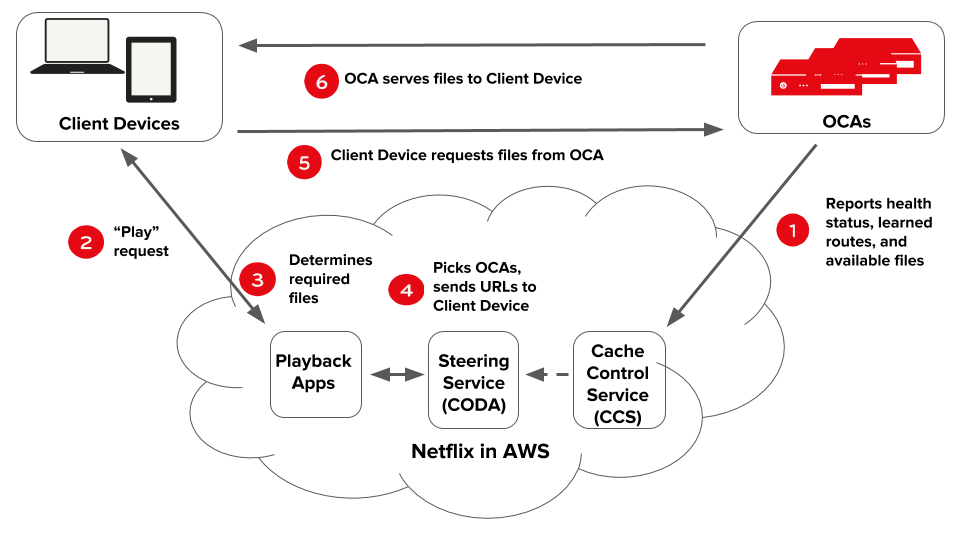
\includegraphics[width=\columnwidth]{img/playback.png}
  \caption{Playback process diagram. \cite{netflix_oca}}
  \label{fig:playback}
\end{figure}

Above is illustrated the process of retrieving content whenever a user wants to
play a Netflix title. OCAs \emph{Open Connect Appliances} are purpose-built
servers responsible to store and serve video files over HTTPS to client
devices.  OCAs as Netflix claims, do not store client data (DRM info or member
data), but only report health metrics to Netflix monitoring services in AWS.

Whenever a play request is issued by a client device, playback application
services in AWS determine which streaming assets are required to handle the
streaming of the intended title

Then the steering service uses cache-control services to select the best OCAs
depending on client characteristics and network conditions, generating URLs
that are passed back to the client device, that is now able to "communicate"
with the OCAs.

\todo{insert an example of URL, and explain how ISP cannot associate a URL to a
specific title in a trivial way}

Netflix partners with ISPs in the deployment of their CDN, following are
presented two different policies:

\begin{figure}[!htb]
  \centering
  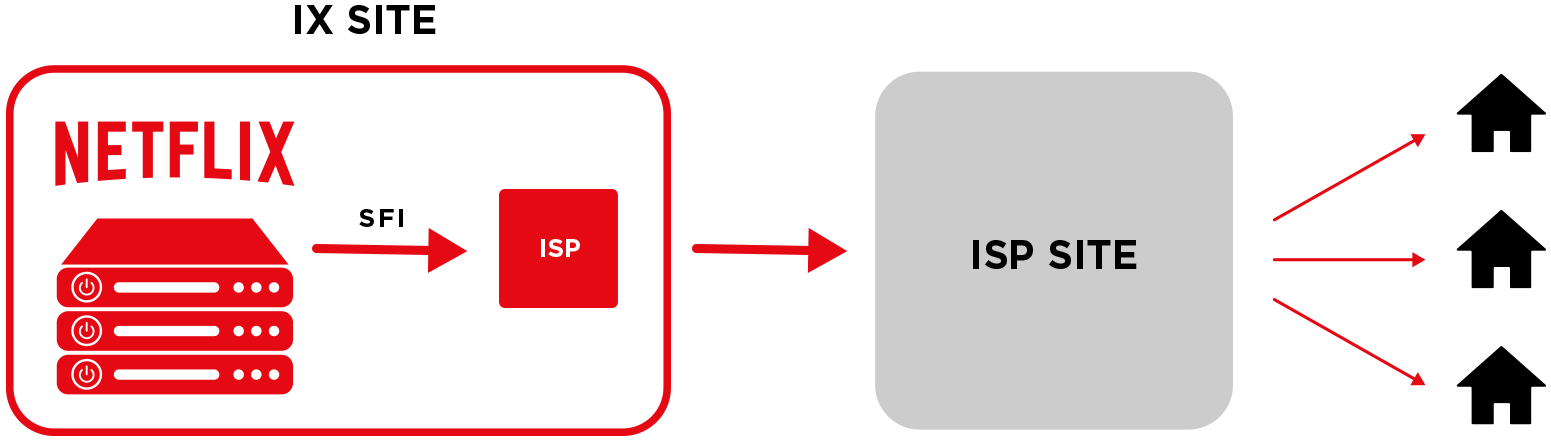
\includegraphics[width=\columnwidth]{img/oca_1.png}
  \caption{OCAs are installed within Internet Exchange Points (IXP), and
  interconnected to ISPs. \cite{netflix_oca}}
  \label{fig:oca_1}
\end{figure}

\begin{figure}[!htb]
  \centering
  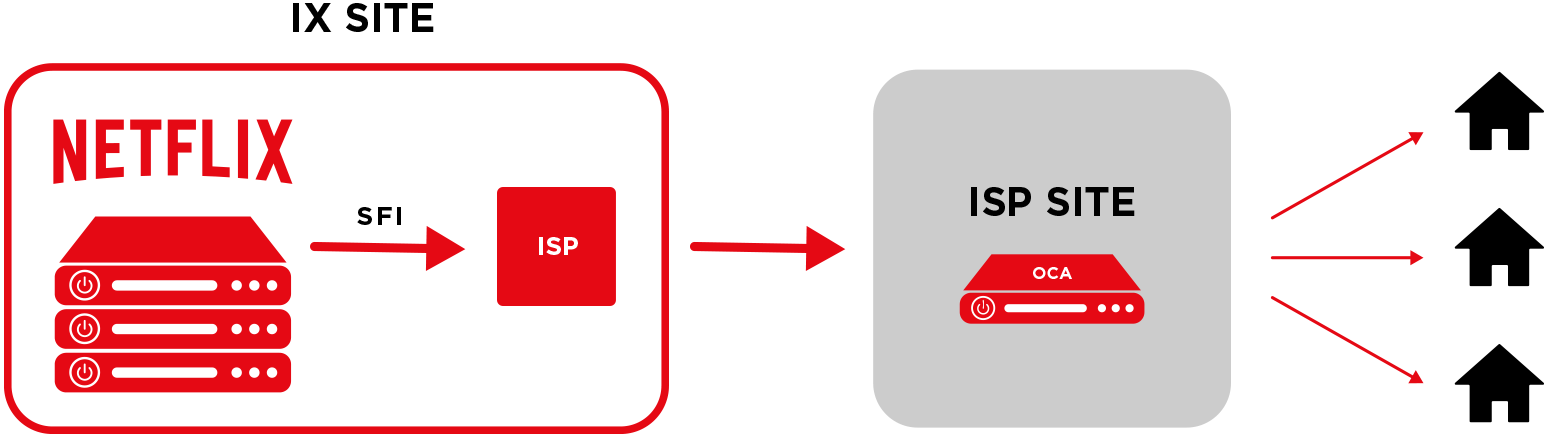
\includegraphics[width=\columnwidth]{img/oca_2.png}
  \caption{OCAs are directly deployed inside ISP networks. \cite{netflix_oca}}
  \label{fig:oca_2}
\end{figure}

\section{Attack Scenarios}\label{attack_scenarios}

Given the nature of modern Internet infrastructure, an adversary interested in
eavesdropping a particular communication, only needs to compromise a node on
the path the communication travels through. An \emph{on-path} attacker could
easily gain passive access to network and transport layers, and start capturing
network traffic. This can include malicious or compromised Wi-Fi access
points, routers, tapped network cables and ISPs. 

Rather than just attacking physical devices, leaks of information could occur
in network connections, in which an attacker physically close to the victim,
could make use of a \emph{Wi-Fi sniffer} to estimate traffic by capturing
physical layer WLAN packets.  Information may be encrypted by 802.11, and the
sniffer may not take into account packet retransmissions at the session layer
nor multiple TCP/IP flows on the same link, potentially causing noise on the
observation. Despite so, Reed et Al. \cite{leaky_streams}, have shown that it
is still possible to estimate WAP-to-client throughput and use it to identify
the content being streamed.

In addition to the above, \emph{side-channel eavesdropping} can exploit
information about the network structure, to saturate a link between the user
and the server, and estimate fluctuations of congestion by sending probes
remotely and observing queueing delays in routers \cite{side_channel}. 

We will now present the relevant phases and tools needed for an ISP to perform
an attack, considering the ISP an \emph{on-path} attacker.

\section{Video Fingerprinting}

In order to identify video stream traffic of a specific user, the ISP needs to
build a database of video fingerprints to match against. To build such a
database, the ISP needs to have access to a network interface, control its
inbound bandwidth, (to get different levels of quality for each title), and
capture incoming traffic passing through it.

In order to control the incoming bandwidth, the ISP could either limit it
directly onto a generic L4 switch, or decide to connect
any UNIX-like machine and throttle the throughput of its main ethernet
interface. We will consider the scenario in which the ISP limits the bandwidth
of the ethernet interface of the switch, (less noisy and more stable).

The value of the enforced bandwidth determines the quality (bitrate) of the
content that will be captured. Assuming that each title has a unique bitrate
ladder, the ISP should come up with an ad-hoc policy for every video to
faithfully reconstruct the quality levels of it. While correct, a more viable
approach to this problem, would be to just consider a range of bitrates capable
of spanning the space of possible quality levels. 

In our own version of the attack, presented in \Cref{sec:approach}, we use
the values in \Cref{tab:bandwidths}. 

\begin{table}[htb]
  \centering
  \begin{tabular}{|c|c|c|c|c|c|c|c|c|c|c|c|c|}
    \hline
    \multicolumn{13}{|c|}{\textbf{Bandwidth levels (Mbps)}} \\
    \hline
    0.6 & 0.8 & 1.2 & 2 & 3.5 & 4.2 & 4.8 & 5.5 & 6.5 & 7.05 & 10 & 15 & 20 \\ 
    \hline
  \end{tabular}
  \caption{Enforced bandwidth levels.}
  \label{tab:bandwidths}
\end{table}

The ISP can now connect a UNIX-like machine to the switch's network interface
with bandwidth limit \emph{b}, and invoke \texttt{adudump} to infer the size of
each \emph{application data unit} ADU by processing TCP/IP packet header
traces that generate \emph{a-b-t} connection vectors \cite{hernandez}.

\subsection{The \emph{a-b-t} model}

The lifetime of a TCP endpoint that sends and receive data units is not only
dictated by the time spent on these operations, but also by quiet times in
which the TCP connection remains idle, waiting for upper layers to formulate
new demands. Clearly, longer lifetimes may have a huge impact overall, due to
the fact that resources needed to handle TCP state, remain reserved for a
longer time. In contrast, ADUs that are sent within a short period of time, get
aggregated by the TCP window mechanism, reducing the exchange of
requests/responses between source and destination.

These ideas have been formalized into the \emph{a-b-t model}, that describes
TCP connections as sets of ADU exchanges and quiet times. The term a-b-t is
descriptive of the building blocks of the model: \emph{a-type} ADUs, sent from
the connection initiator to the connection acceptor, \emph{b-type} ADUs, sent
from the responder back to the initiator, and quiet times \emph{t}'s, during
which, no data segments are exchanged.

The model has two different flavors depending on whether ADU interleaving is
sequential or concurrent: the former is used for modeling connections for which
only one ADU is sent from one endpoint to the other at a given point in time,
(one endpoint will wait until the other has completed the transmission of the
current ADU before sending a new one), while the latter is used for modeling
connections in which both endpoints send and receive ADUs simultaneously.

As one can notice from a sample traffic trace from Netflix, the two endpoints
behave in a sequential fashion, as shown by the \texttt{SEQ} flag in
\Cref{lst:adutrace}.

\begin{adu}[caption={Incoming traffic trace of Mulan, captured at 10Mbps (first 10 segments).}, label={lst:adutrace}]
ADU: 1565880580.152388 192.168.0.157.54924 <1 45.57.19.134.443 198837 SEQ 0.804088
ADU: 1565880581.321246 192.168.0.157.54924 <1 45.57.19.134.443 198760 SEQ 0.907568
ADU: 1565880582.688335 192.168.0.157.54924 <1 45.57.19.134.443 199407 SEQ 1.052862
ADU: 1565880591.912352 192.168.0.157.54974 <1 45.57.19.134.443 525046 SEQ 0.058709
ADU: 1565880592.168340 192.168.0.157.54968 <1 45.57.19.134.443 275568 SEQ 0.558654
ADU: 1565880592.168344 192.168.0.157.54974 <1 45.57.19.134.443 305115 SEQ 0.062028
ADU: 1565880592.172495 192.168.0.157.54982 <1 45.57.19.134.443 198735 SEQ 0.670224
ADU: 1565880592.697314 192.168.0.157.54974 <1 45.57.19.134.443 236474 SEQ 0.179115
ADU: 1565880592.820292 192.168.0.157.54982 <1 45.57.19.134.443 286547 SEQ 0.106913
ADU: 1565880592.820395 192.168.0.157.54968 <1 45.57.19.134.443 198530 SEQ 0.310506
\end{adu}

\subsection{Inference}

\begin{figure}[!h]
  \centering
  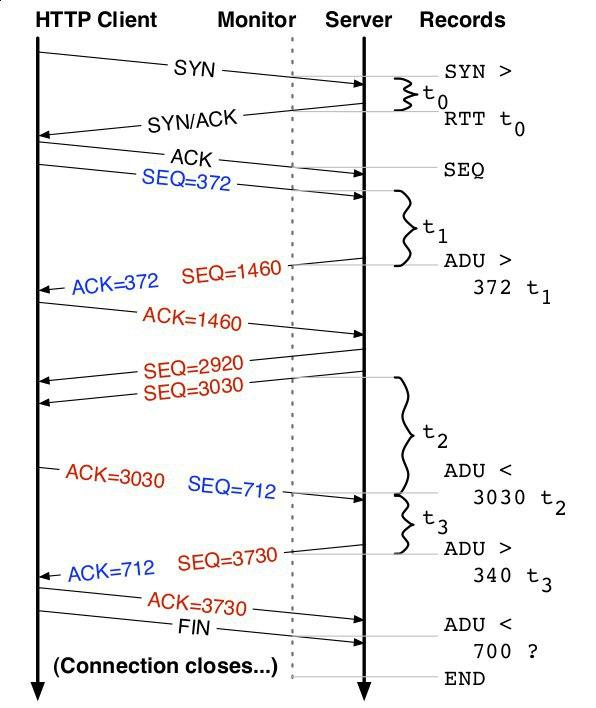
\includegraphics[width=0.6\columnwidth]{img/adudump.png}
  \caption{Detailed segment size inference in adudump.}
  \label{fig:adudump}
\end{figure}

\Cref{fig:adudump} shows an example of how Adudump's inference process works.
The connection starts when the three-way handshake completes, (marked as a
\texttt{SEQ} record). The monitor then records the time the first data segment
is sent from the client. The server then acknowledges the previous request, and
adudump infers the size of the completed ADU to be 372 bytes, generating a
record with the ADU's size direction and think-time. Note how adudump generates
no record until it infers that the ADU is complete, moreover the think times
reported, are relative to the position of the monitor in the network, the
farthest the monitor is from the server, the noisiest the measure of quiet
times becomes. More on the effect of quiet times is described in
\Cref{sec:approach}.

\subsection{Identifying Netflix traffic}\label{dns}

In order to identify specific video traffic from a Netflix CDN, the ISP could
either inspect the DNS response packets or the TLS handshake messages, and
perform a DNS lookup for each video every time, or to maintain an updated list
of IP addresses with mappings to the recorded traffic. Then all the ISP is left
with, is a mixed trace of audio and video segments. Each Netflix audio segment
represents about 16 seconds of playback, while every video segment corresponds
to a 4 second playback. The ISP could now decide to either filter out audio
segments by either thresholding on the size of ADUs, as done by Reed et Al (at
200 kilobytes), or to consider audio as part of the fingerprint of a title. The
200 kilobytes threshold represent a good heuristic when considering traces
recorded at high bandwidth levels, in fact, audio segments sizes are around 198
kilobytes, whereas if considering the same title at a low level of bandwidth
(less than 1 Mbps indicatively), one cannot distinguish audio and video
segments by their size. For this reason, we consider an approach that does not
filter out audio segments. In \Cref{sec:approach} we highlight the difference
between the two methods.

\subsection{Building a database of fingerprints}

The ISP can now automate the streaming of Netflix videos, and build a database
of such fingerprints. Here, the ISP is free to use a method of storage of
choice, depending on the granularity of the features required to represent each
title, and on the cardinality of the set of titles it wants to capture.  In
addition, as Netflix is constantly adding/removing titles from its library, the
ISP is required to constantly keeping updated the database to guarantee that
the attack can target newly added titles.

\section{Capturing video traffic}

In order to capture video traffic to match it against a database of collected
fingerprints, it requires the ISP to be in possess of a generic L4 switch
capable of mirroring traffic from a port to another one. Then any UNIX-like
system that implements \emph{libpcap} is suitable for capturing inbound traffic
on the mirrored port, as presented below in \Cref{fig:schema}.

\todo{modify this image}

\begin{figure}[!htb]
  \centering
  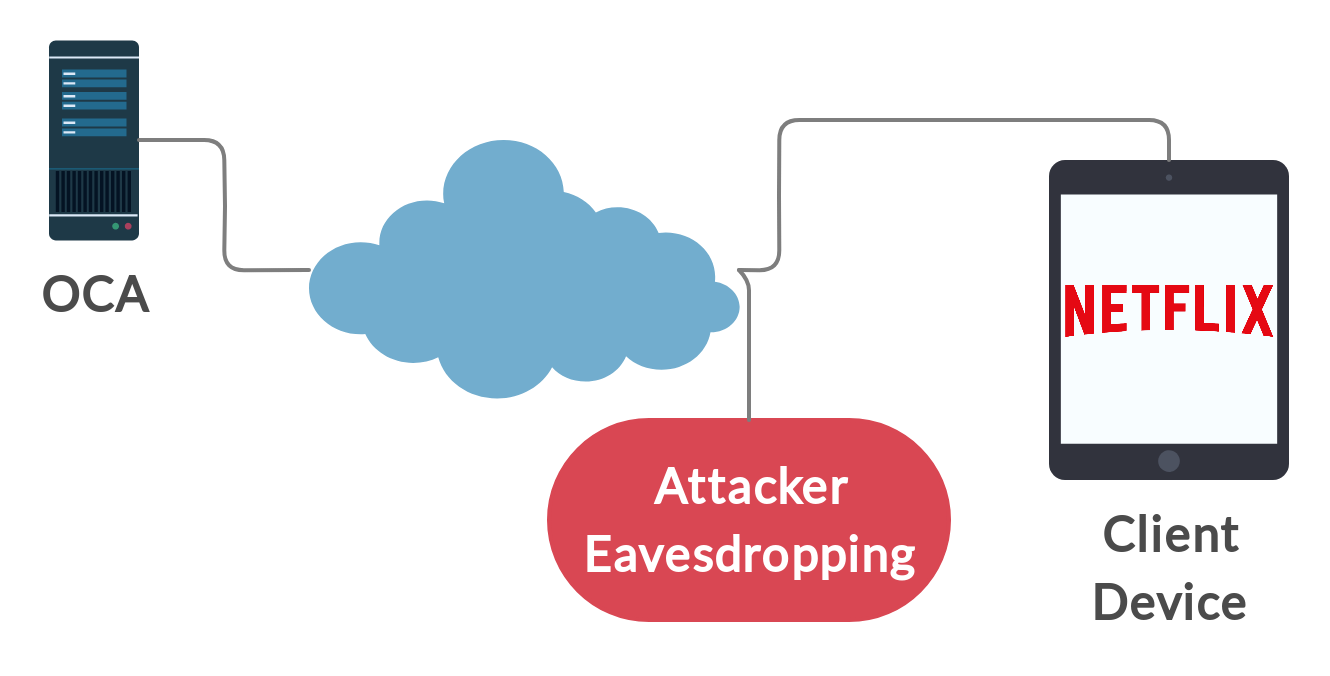
\includegraphics[width=\columnwidth]{img/schema.png}
  \caption{Traffic capture scenario.}
  \label{fig:schema}
\end{figure}

In this scenario, the client is unaware of the fact that its traffic is being
mirrored and recorded by the ISP, and there is no practical way for him to
claim that. On the other hand, a user concerned with its privacy, may avoid
such attack, as described in \Cref{sec:vpn}.

\subsection{Data acquired by the ISP}

Captured traffic, as shown in \Cref{lst:adutrace}, apart from the size of each
segment and quiet times, include timestamps of each ADU, and source and
destination IP addresses. With this information, the ISP is able to reconstruct
streaming habits of every targeted user (identifiable by the source IP
address),  by looking at what time he/she does usually connect to the platform,
identifying the content of the stream (matching to fingerprints), and by
analyzing how much time the user spends watching content. Thus the ISP can
aggregate user's collected data and build a database of user profiles to use it
for its own will. Data about a particular user is no longer in the solely hands
of Netflix, as one could argue it should be, but it now resides in some ISP
database, potentially exploitable and profitable, with any prior consent.

\subsection{Matching Captured traffic to fingerprints}

The ISP can now identify the captured trace by comparing it to the saved
fingerprints.  Based on the type of data structure used to store them, there
are several methods to search and retrieve the best candidate for a given
trace. We will not articulate this process here, but we rather present our own
solution later in \Cref{sec:approach}.

\subsection{Possible countermeasures}\label{sec:vpn}

In order to safely stream Netflix videos without the ISP being able to identify
the content of them, a user particularly concerned about its privacy, (e.g.
public figures, politicians, government agency employees), may decide to use a
VPN. When using a VPN, the user, still needs the ISP to connect to the
internet, but instead of having the ISP communicating directly with the desired
resource, the ISP now "talks" with the VPN server. It is responsibility of the
VPN server in fact, to establish a communication with the webpage the user
wants to access.  The key point is that the client and the VPN server establish
a secure connection (VPN tunnel). Thus, as long as the user's VPN of choice,
encrypts data transfer, either with IPSec's \textbf{Encapsulated Security
Payload} or, in case of a remote-access VPN, with point-to-point based
protocols such as L2F, PPTP or LT2P, the user is guaranteed that its traffic
cannot be intercepted by the ISP. This is feasible as long as both the VPN
software provides an automatic kill switch to avoid dropouts, and the online
resource does not restrict access to users connected via VPN. 

Netflix does not allow the use of VPN software to prevent users to get access
to other countries catalogue, although certain VPN clients are able to bypass
this check \cite{nordvpn}.

\chapter{Approach}\label{sec:approach}

We will now present our contribution and practical approach to build a database
of fingerprints and to capture and identify video traffic of an unaware user
over a compromised network.

We have built a system capable of manipulating the incoming bandwidth of a
network interface, able to obtain fingerprints for a limited number of Netflix
titles at various enforced bandwidth levels, and reconstructed each video's
bitrate ladder. We compare our reconstructed bitrate ladders with the bitrate
ladders constructed from HTTP header (HARs), and report, for each one its the
RMSE.  Eventually, we evaluate the robustness of the saved fingerprints, by
feeding to our identification mechanism, several test-captures of video IDs
(present in our fingerprint's database), at \emph{unseen} bandwidth levels. In
this phase we study the impact of tuning the parameters of the system in
relation to the number of successfully/unsuccessfully identified videos, and
report relevant statistics of each test.

\section{Attack Scenario}

Our own version of the attack, conversely to the one depicted in
\Cref{fig:schema}, does not include the ISP as a potential adversary, nor does
involve an attacker that has compromised an ISP CDN.  We consider a specific
case in which the attacker is a malicious user \emph{i}, with access to the
same network an honest client is using to stream a Netflix title. Attacker
\emph{i} has:

\begin{itemize}
    \item either installed a passive TAP device on a LAN
    \item or gained control of the main switch of a LAN
    \item or compromised an AP over a public WiFi network.
\end{itemize}

For each of the aforementioned scenarios, the steps required for the attacker
\emph{i} to identify video traffic of another user, are the same: the first
phase consists of recording fingerprints of each Netflix title, process them,
store them in a persisent (and convenient for search and retrieval) data
structure, while the second phase consists of exploiting the compromise device
in the network to capture user's traffic and identify the content of the stream
by querying the database of fingerprint.

\section{Video Fingerprinting}

Let $T$ be the set of Netflix titles for Switzerland, we refer to $n$ as the
cardinality $|T|$, which is roughly 3500; consider now the set $R$ as the set of
bandwidth levels shown in \Cref{tab:bandwidths}, we refer to $i$ as the
cardinality $|R|$.

Consider now the cartesian product $T \times R$:

\begin{equation*}
T \times R = \{(t_1, r_1), (t_1, r_2) \dots (t_n, r_i)\} 
\end{equation*}

and its cardinality:

\begin{equation*}
|T \times R| = |T| \cdot |R| = n \cdot i \approx 45500
\end{equation*}

Due to time restrictions, we have decided to fix the size of the set $T$ of
titles to 100, in order to give a proof of concept on the feasibility of such
an attack.  According \cite{netflix-real-time}, we have also decided to bound
the time of each video capture to 4 minutes of playback, as it has been shown
to be sufficient in order to uniquely identify a video over more than 40000
titles.

\subsection{Implementation overview}

We have implemented a set of Python scripts to be able to:

\begin{enumerate}
    \item Crawl the swiss Netflix catalogue to obtain a list of video IDs.
    \item Manipulate the incoming bandwidth of an ethernet network interface.
    \item Invoke \texttt{tcpdump} listening on the same network interface.
    \item Instrument the browser to:
        \begin{enumerate}
            \item Navigate to a specific title URL (identified by the title ID).
            \item Control the Netflix video player by injecting JavaScript code.
            \item Capture HAR metadata via a proxy.
        \end{enumerate}
\end{enumerate}

Note that contrary to \cite{netflix-real-time}, in this phase we do not make
use of adudump, instead, to record traffic, we use tcpdump \cite{libpcap}. The
main reason behind this choice, is the fact that adudump has been conceived to
reconstruct data segments sizes in an online fashion. By doing so, the time
spent by adudump processing each segment, creates an overhead that in turn,
results in noisy measurements.  Adudump can work in an offline-fashion, simply
by passing as input a \texttt{pcap} \cite{libpcap} file, that gets generated
when invoking tcpdump.  We have tested and analyzed this behaviour and visual
evidence is presented in \Cref{fig:online_vs_offline}.

\todo{add plots of adudump's behaviour when invoked online vs on a .pcap file}

\subsection{Crawler}

The script responsible of crawling the Netflix catalogue is
\texttt{crawler.py}.  We use the \texttt{scrapy} Python library \cite{scrapy}
to get a list of Netflix titles divided by genre. Note that, for the sake of
simplicity, we have decided to work only with movies, as for TV series, we
would have need to add checks due to the autoplay function of subsequent
episodes in the viewing phase.

The resulting output of the script is a CSV file with the following structure:

\begin{adu}[caption={Sample of crawled movies}, label={lst:crawl_output}]
ID        GENRE             TITLE

70115629, Family Animation, Despicable Me
70264803, Family Animation, Despicable Me 2
80096067, Family Animation, Ice Age: Collision Course
70220028, Family Animation, Hotel Transylvania
80121840, Family Animation, The Emoji Movie
70021636, Family Animation, Madagascar
70216224, Family Animation, Madagascar 3: Europe's Most Wanted
70213513, Family Animation, Brave
14607635, Family Animation, Mulan
\end{adu}

Due to the fact that a movie can be labeled in more than one category, the
resulting CSV have been filtered to include just one occurrence of each title.

\begin{bash_script}[caption={Command to filter out unique IDs}, label={titles}]
cat netflix_titles/titles.csv | cut -d , -f1 | sort | uniq
\end{bash_script}

\newpage
\subsection{Bandwidth Manipulation}

In order to be able to manually control the bandwidth of the ethernet
interface, we use \texttt{tcconfig} \cite{tcconfig}, a Python wrapper for the
\texttt{tc} \cite{tc} Unix utility to configure traffic control in the kernel.

The script that throttles the bandwidth is \texttt{bandwidth\_manipulator.py},
that invokes the command:

\begin{bash_script}[caption={Enforce a bandwidth rate on the specified interface}, label={tcconfig}]
tcset --device <network_interface> --direction incoming --rate <bandwidth_rate>
\end{bash_script}

\subsection{Tcpdump}

The script that records the capture traffic is \texttt{capture.py}, it calls
tcpdump as below:

\begin{bash_script}[caption={Listens for TCP/IP traffic on the specified
    interface}, label={tcpdump}]
tcpdump -i <network_interface> net 45 -w <output_file>
\end{bash_script}

Note the usage of argument \texttt{net 45}. As Netflix OCAs IP addresses are of
the form \texttt{45.XXX.XXX.XXX}, to simplify the process of identifying
traffic from Netflix, we just use this regular expression for convenience.
Steps required to carry out a more general way to achieve this have been
described in \Cref{dns}.

\subsection{Automated streaming with Selenium}

In order to instrument the browser to automatically stream each title, we have
developed a script that uses the \texttt{Selenium} library \cite{selenium}.
Selenium provides a \texttt{WebDriver} interface capable of controlling various
browsers such as Chrome, Opera, Safari, Firefox and others. One must use the
appropriate version of the WebDriver, according to the browser of choice and
its version. For convenience of use, and support, we have chosen to work with
GoogleChrome and its ChromeDriver interface.

In order to asses the quality of adudump's inference of video segment sizes, we
compare the recorded traffic with HAR \cite{har} metadata. The format of each
HAR file is a json object containing content and session data acquired by the
browser during the playback of the video. For this task, we use
\texttt{Browsermob} \cite{browsermob}, a webproxy built to work with Selenium.

Furthermore, to speedup the capture of each video, we have installed an
extension that is able to control HTML5 video speed playback.

\newpage
We have implemented a class \texttt{netflix\_browser.py} capable of:

\begin{enumerate}
    \item Log in the user to its Netflix account
    \item Navigate to a video url given a video ID
    \item Start the proxy to record HAR metadata
    \item Seek the video to 240 seconds (4 minutes) (avoiding entry credits)
    \item Wait until the buffer of the video reaches 8 minutes (start at 240
        seconds, ends at 480).
    \item Stop the proxy and save the resulting HAR file
\end{enumerate}


\section{Post-processing}

The script that handles post-processing of \texttt{.pcap} output files is
\texttt{post\_process.sh}. It is composed by three main functions.

The first one invokes adudump on the traces recorded with tcpdump, after that,
it extracts the DNSs contained in the HAR metadata and performs a DNS lookup
using Unix's \texttt{host} command. This step is required to get the complete
list of IP addresses of the OCAs that served the video, so that we can filter
all non-video traffic that tcpdump has captured. In addition we threshold ADUs
which sizes are less than 100 kilobytes, as mentioned in \Cref{dns}.

The second function is responsible for generating the bitrate ladders of each
title, and to save all fingerprints in a text file. Given a trace at a
particular bandwidth level $b$, we compute the average bitrate as:

\begin{equation*}
    AVG_{bitrate} = \dfrac{8}{4} \cdot \dfrac{\Sigma_{i=0}^{n} \hspace{2pt} adu_i}{n}
\end{equation*}

We average over all ADUs (sizes are in bytes), divide by 4 seconds (approximate
lenght of a video segment according to \cite{netflix-real-time}), and multiply
by 8 to get a measure in \emph{bits/s}. 

We repeat the process decribed above, also by generating fingerprints from the
HAR records we capture with our proxy. By doing so, we can reconstruct the
\emph{true} bitrate ladders, for each capture, and use them as a term of
comparison to asses the quality of the ADU's reconstruced ladders. For each
ADU reconstructed bitrate ladder, we compute the \emph{mean-normalized} RMSE
with the HAR reconstructed ones as shown in \Cref{sec:rmse}.

\begin{figure}[!h]
  \centering
  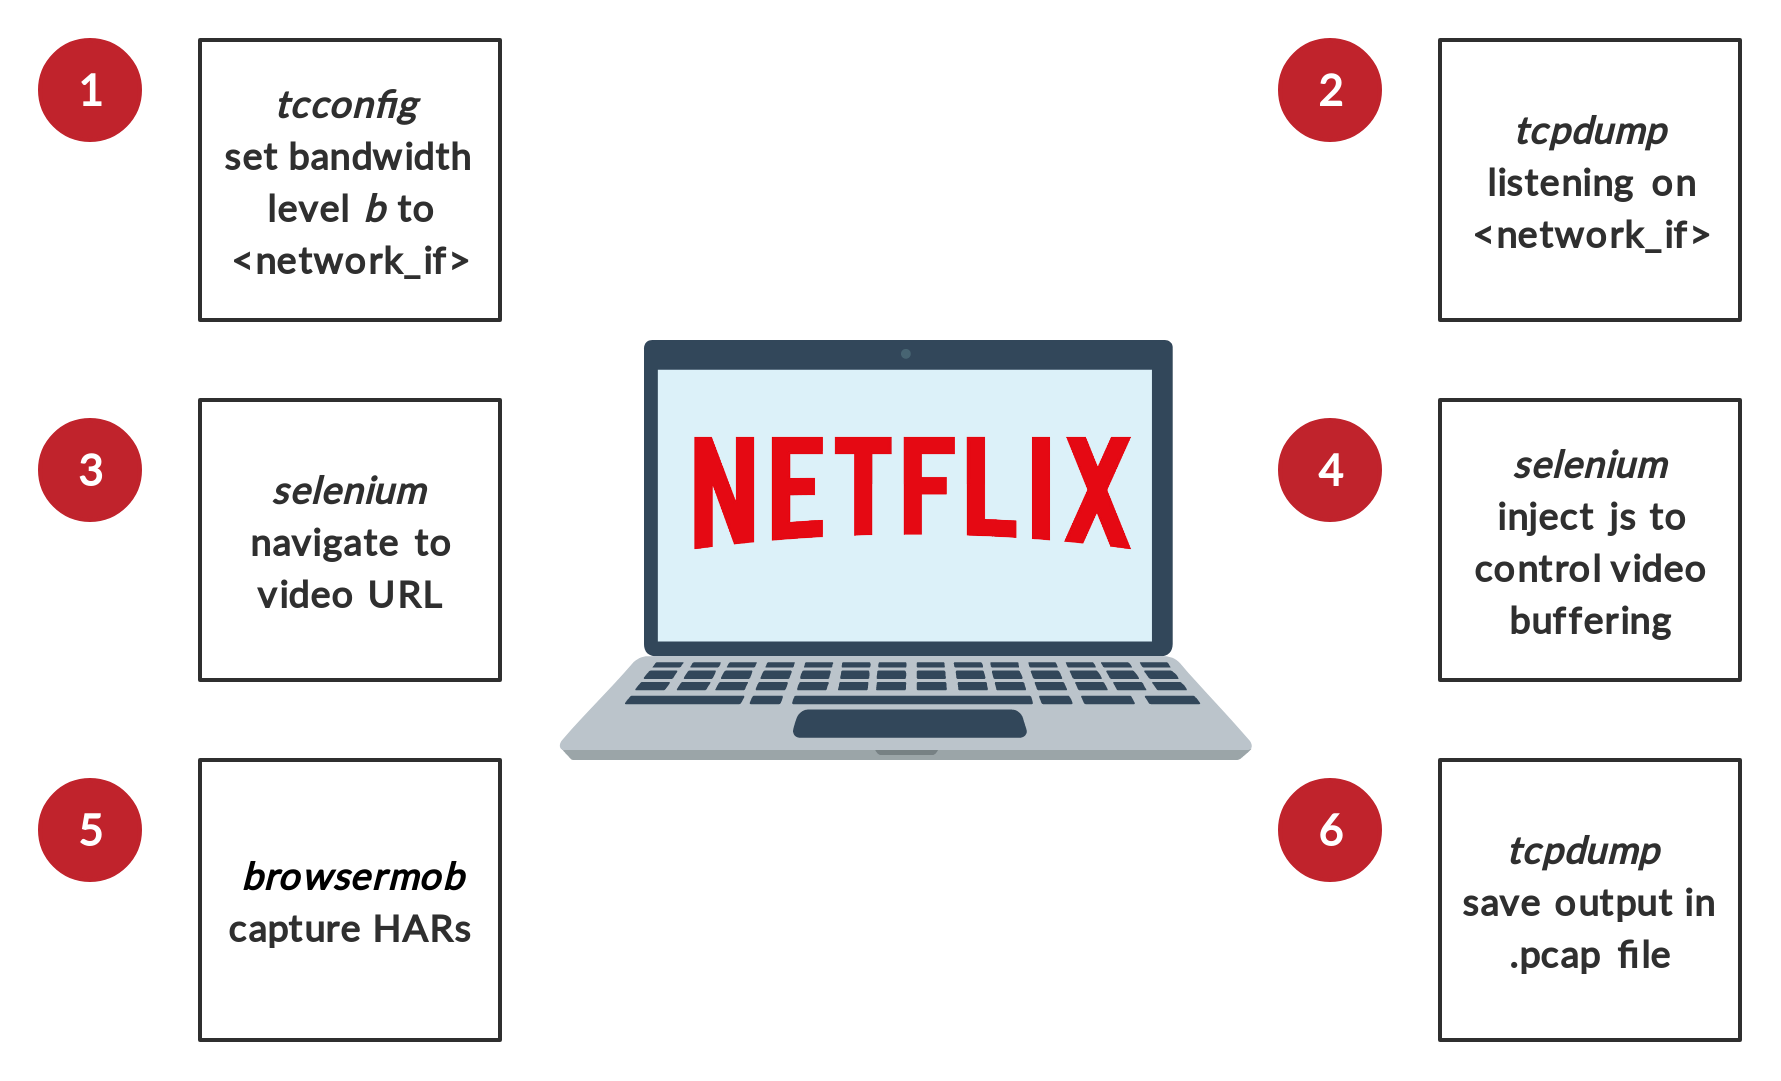
\includegraphics[width=\columnwidth]{img/fingerprints.png}
  \caption{Overview of the process of acquiring video fingeprints.}
  \label{fig:fingerprints}
\end{figure}


\section{Capturing video traffic}\label{sec:testing}

In order to evaluate the attack, we capture a set of video traffic traces (the
ones the attacker $i$ can retrieve by mirroring traffic on the compromised
device), at unseen enforced bandwidths. In practice, our database of
fingerprints hosts 100 movie titles at the 13 bandwidth levels presented in
\Cref{tab:bandwidths}, while the new \emph{unseen} bandwidths are listed below
in \Cref{tab:unseen_bandwidths}.

\begin{table}[htb]
  \centering
  \begin{tabular}{|c|c|c|c|c|c|c|c|}
    \hline
    \multicolumn{8}{|c|}{\textbf{Unseen Bandwidth levels (Mbps)}} \\
    \hline
    0.5 & 1.0 & 3.0 & 5.0 & 6.0 & 8.0 & 12.0 & 18.0 \\
    \hline
  \end{tabular}
  \caption{Enforced unseen bandwidth levels.}
  \label{tab:unseen_bandwidths}
\end{table}

As for the acquisition of fingerprints, we repeat the same exact steps to build
our testing set, that is composed by the same 100 titles recorded at the new 8
unseen bandwidth levels depicted above. 

\newpage
\section{Identification}

For this purpose, we have implemented a modified version of the search tree
used in \cite{netflix-real-time}. All the scripts in this Section can be fuond
under the \texttt{identify} directory located at the root of the project.

The identification process involves two parties: a Java program that runs as
a proxy to our database, and a Python script that takes as input the
fingerprints of captured traffic to query the database for matches.

The Python script queries the Java process running the KD-tree, that returns a
list of possible matches for the given captured trace.

%\begin{figure}[!h]
  %\centering
  %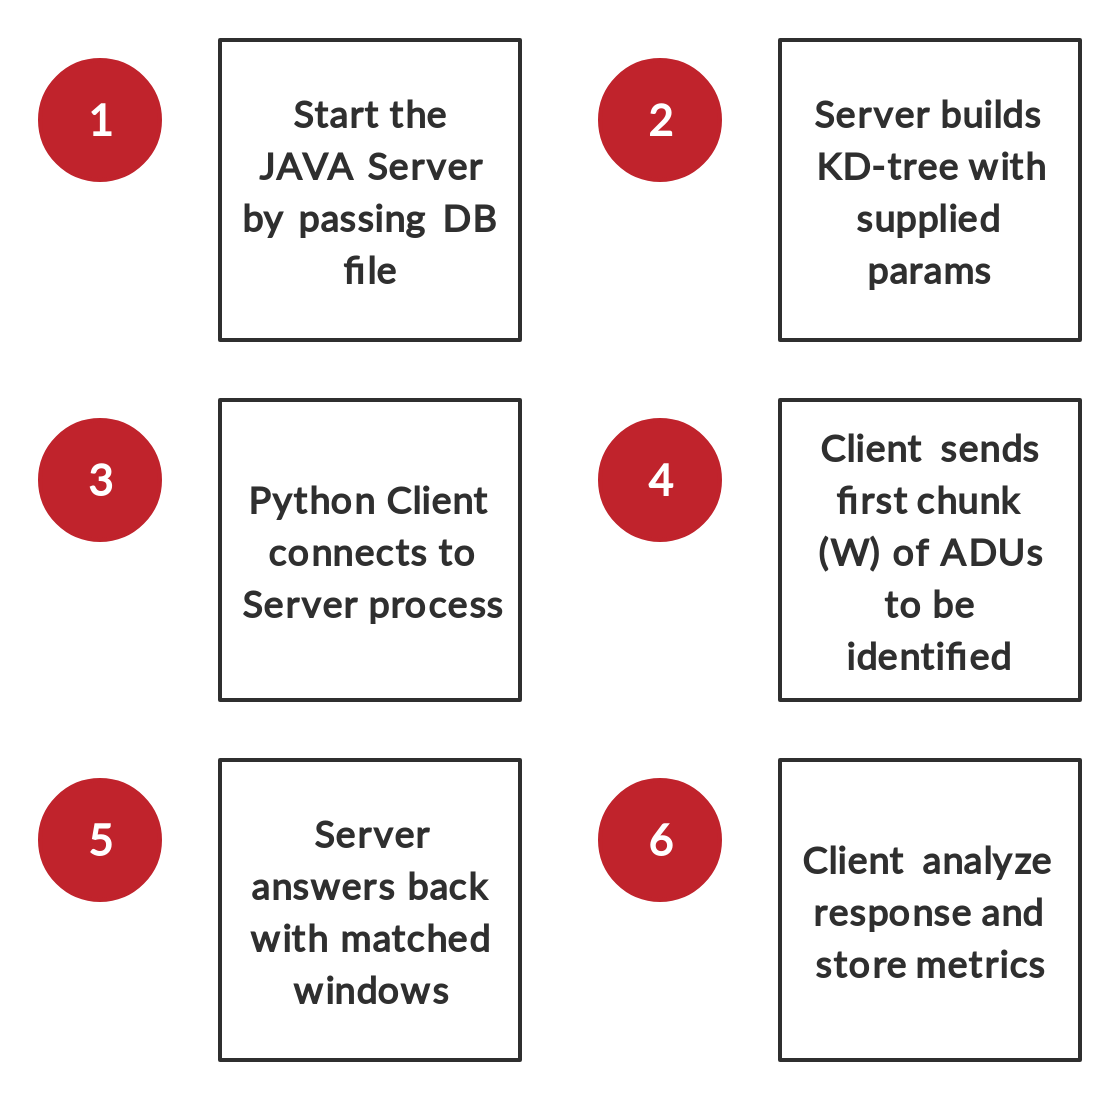
\includegraphics[width=.6\columnwidth]{img/identification.png}
  %\caption{Overview of the process of identification.}
  %\label{fig:identification}
%\end{figure}

\subsection{KD-Tree}

The code that implements the KD-Tree is found under the \texttt{identify/server}
directory. \texttt{runServer.sh} runs an instance of the system and requires 6
parameters as input:

\begin{bash_script}[caption={Start the Java Server}, label={lst:java}]
        cd server && ./runServer.sh <db_file> <capture_file> <window_size> <key_size> <key_mode> <key_delta> <pearson_threshold>
\end{bash_script}

To simplify writing, we assign to the following parameters a corresponding greek letter:

\begin{itemize}
    \item $\omega$ represents the window size.
    \item $\kappa$ is the key size. 
    \item $\mu$ reprents the key mode.
    \item $\delta$ represents how broad the search it will be.
    \item $\rho$ represent the minimum pearson correlation coefficient to accept a match.
\end{itemize}

The above script executes \texttt{Netflid.jar}, composed by the following
Java classes:

\begin{itemize}
    \item \texttt{Netflid}: main Class, sets up the \texttt{KDTree}, and start a
        \texttt{ServerThread} instance.
    \item \texttt{KDTree}: implements the KD-tree data structure.
    \item \texttt{ServerThread}: listens for the client to send data, queries
        the \texttt{KDTree}, and respond to the client with matches.
    \item \texttt{Window}: constructs and store the key to search the \texttt{KDTree}.
    \item \texttt{Movie}: represents a movie instance.

\end{itemize}

\subsection{Building the KD-Tree}

\texttt{Netflid} is the main class that creates a \texttt{KDTree} instance
(with $K$ being the dimension of the search key), to which every record in the
database is added to. Each record, has the following structure:

\begin{bash_script} 
ID              AVG_BITRATE  SEGMENTS
896970_15000    3038         321427,198559,113973 ...
\end{bash_script}

The \texttt{ID} of the record is formed by the video ID, and the
enforced bandwidth at which the title has been captured
(\texttt{896970\_15000}), represents movie ID 896970 \emph {Red Heat},
recorded at 15.0 \emph{Mbps}. Note how the number of segments for each
record is not fixed, as explained in \Cref{sec:problems}.  For each
record, we create an instance of \texttt{Movie}, in which we store its
ID, the average bitrate and its segments. Based on the number of
segments $s$, we build $s-1$ \texttt{Window}s of $\omega$ segments.
For each window, we build a search key of dimension $K$, in one of the
following modes, expressed by $M$: 

In case $M$ \texttt{== 0}, the key gets constructed by assigning the
total sum of the segment sizes in the window as first dimension; the
rest $K - 1$ dimensions, represent the proportion of data received
within $\dfrac{\omega}{K-1}$ segments with respect to the
aforementioned total in the first dimension.

In case $M$ \texttt{== 1}, instead we store the average bitrate
(computed as in \Cref{sec:idk}) of all segments in the window as
first dimension, then each of the $K-1$ dimensions is the average
bitrate of $\dfrac{\omega}{K-1}$ segments, normalized again by the
first dimension.

\subsection{Querying the KD-Tree}

The script acting in the role of the client, is located under \texttt{identify/client}'s directory

\begin{bash_script}
cd client && cat <capture_file> | grep ADU | awk '$6 > 100000' | cut -d " " -f2,3,4,5,6 | python preprocessor.py | python detector.py 127.0.0.1 1007 <capture_file> <window_size> <key_mode> <key_delta>
\end{bash_script}

After having added the key to the \texttt{KDTree}, we start a
\texttt{ServerSocket} thread that listens for incoming connections from the
client. \texttt{ServerThread} is the runnable class responsible for consuming
the input of the socket the Python client communicates through. 

The Python Client consists of a script that takes as input a post-processed
traffic capture, and sends sliding window of $\omega$ segments until it has
consumed all lines.

The \texttt{ServerThread} in Java reads up to $\omega$ lines, and creates a
\texttt{Window} and its corresponding key with the same method used when adding
records from the database to the \texttt{KDTree}. Then it queries the
\texttt{KDTree} by generating an upper, and a lower range key, with the
specified $\delta$ (the greater $\delta$ is, the broader the search will be).
The \texttt{KDTree} then retrieves a list of matching windows with a
\emph{pearson correlation} coefficient greater than $\rho$.

\chapter{Evaluation and Analysis}\label{sec:results}

The scripts that perform the evaluation of our testing set, are \texttt{evaluation.sh} and \texttt{exec\_query.sh}.

\section{Video Identification}
After receiving a list of matching windows from the KD-Tree, we classify each one of them as a proper \textbf{match} iff the window's ID matches the ID of the capture we passed to the Java identification process, whereas, if the ID of the capture and the window ID are different, we classify the returned window as a \textbf{mismatch}.

We then report, for various $\omega$ window sizes, the accuracy of our method, to be the proportion of matches with respect to the number of mismatches over the total number of returned windows as:

Let $n$ be the number of returned windows for a given capture trace, and let $TP$ represent the number of matches, and $FP$ to represent the number of returned mismatches:

It follows that $n = TP + FP$

\begin{equation*}
    \mathbf{acc} = \dfrac{TP}{n} = 1 - \dfrac{FP}{n}
\end{equation*}

As mentioned in \Cref{sec:testing}, our testing dataset consists of the same 100 movies present in the database at 8 unseen enforced bandwidths. We pass each capture to the identification process, that runs the evaluation by varying the window size $\omega$, and the corresponding key size $\kappa$. For every run, we then compute the number of matches/mismatches, and report the statistics shown in \Cref{lst:stats}. In addition, we plot for each configuration the number of matches, the number of collisions and the number of mismatches. The number of collisions, represents the number of matches from different bandwidth levels, (e.g. suppose to have a capture at 6.0 \emph{Mbps}, now assume the KDTree returns as matching windows, a list of matches all of the same movie, but at different bandwidths, 5.0 \emph{Mbps}, and 7 \emph{Mbps}, then the number of collisions is 2).

%\begin{figure}[!h]
  %\centering
  %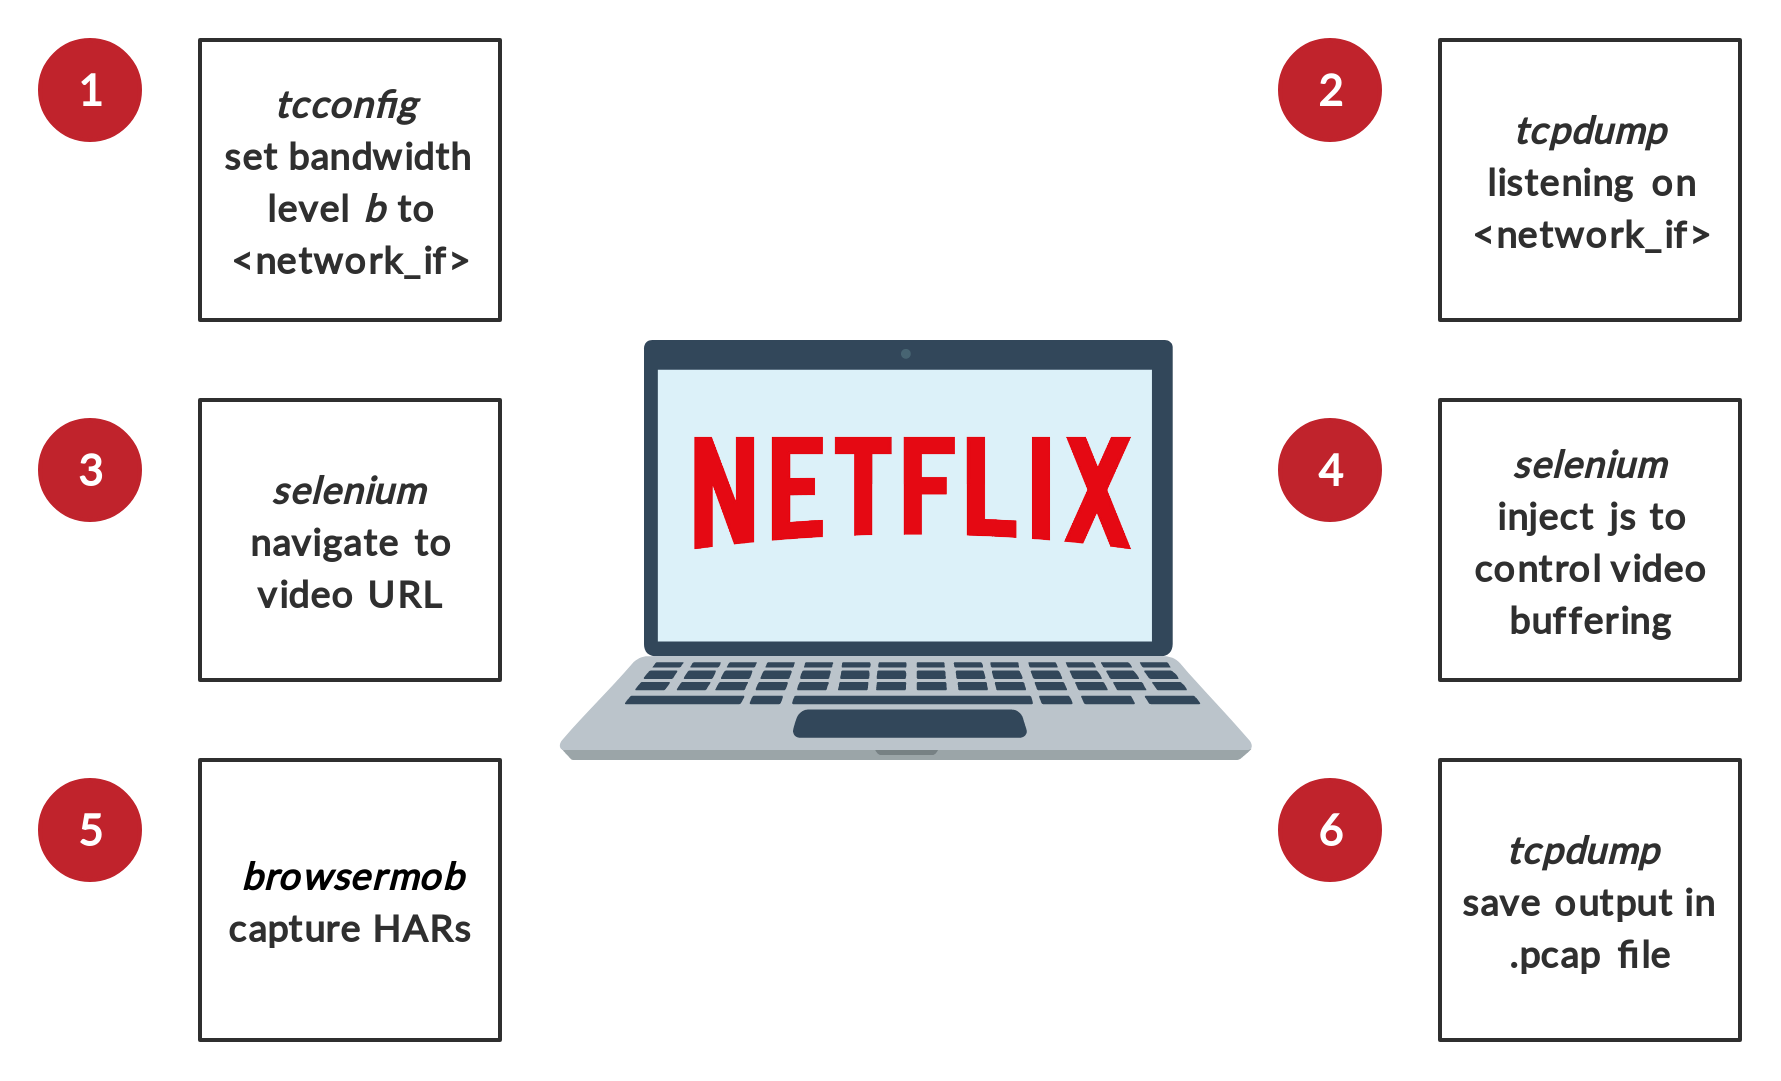
\includegraphics[width=\columnwidth]{img/fingerprints.png}
  %\caption{Overview of the process of acquiring video fingeprints.}
  %\label{fig:fingerprints}
%\end{figure}

\section{Bitrate Ladders}

At first, we evaluate the accuracy of the reconstruced bitrate ladders by computing the RMSE between each one and its corresponding HAR-based bitrate ladder. We have decided to use the RMSE, as it is a well-known indicator that aggregates the residuals to give a measure of the magnitude of error in our predictions, and it is computed as follows.

Let $Y=\{y_1, y_2 \dots y_n\}$ be the set of HAR-based bitrates for movie $m$, at enforced bandwidth
$b$, and let $\hat{Y}=\{\hat{y}_1, \hat{y}_2 \dots \hat{y}_n\}$ be the set of ADU-based computed bitrates for the same
movie at the same enforced bandwidth, then:

\begin{equation*}
    \mathbf{RMSE_{m, b}} = \sqrt{\dfrac{\Sigma_{i=0}^{n}(y_i - \hat{y}_i)^2}{n}}
\end{equation*}

where $n = |Y| = |\hat{Y}|$

Then, the \emph{mean-normalized} RMSE is given by:

\begin{equation*}
    \mathbf{NRMSE_{m, b}} = \dfrac{RMSE_{m, b}}{\overline{\hat{y}}}
\end{equation*}

In addition, in order to assess the uniqueness of both the real and the
reconstrcuted bitrate ladders, we compute, for each bitrate ladder, its average
bitrate, the bitrate standard deviation, and the median.

\begin{small}
\begin{longtable}{|c|c c c|c c c|c|}
    \caption{Collected statistics for the bitrate ladders (values in
    \emph{Mbps})}\label{tab:bitrate_ladders_stats}\\
\hline
\textbf{Title ID} &
\multicolumn{3}{c|}{\textbf{Real}} &
\multicolumn{3}{c|}{\textbf{Reconstruced}} &
\multirow{2}{*}{\textbf{RMSE}} \\
& $\mu$ & $\sigma$ & $\tilde{y}$ & $\mu$ & $\sigma$ & $\tilde{y}$ & \\
\hline
\endhead
\hline
\endfoot
1151721 & 0.77 & 0.25 & 0.92 & 0.73 & 0.27 & 0.88 & 0.09 \\
14607635 & 0.81 & 0.25 & 0.95 & 0.74 & 0.27 & 0.89 & 0.12 \\
328438 & 0.88 & 0.34 & 1.06 & 0.89 & 0.37 & 1.06 & 0.06 \\
60000870 & 1.22 & 0.80 & 1.03 & 1.13 & 0.90 & 0.89 & 0.12 \\
60004481 & 0.75 & 0.19 & 0.85 & 0.65 & 0.19 & 0.76 & 0.16 \\
60020801 & 0.88 & 0.33 & 1.06 & 0.84 & 0.35 & 1.00 & 0.08 \\
60027695 & 0.93 & 0.38 & 1.13 & 0.92 & 0.41 & 1.08 & 0.06 \\
\rowcolor{lightgray}60033314 & 0.45 & 0.03 & 0.46 & 0.30 & 0.06 & 0.34 & 0.50 \\
70019012 & 1.59 & 1.09 & 1.40 & 1.52 & 1.15 & 1.25 & 0.07 \\
70021636 & 0.98 & 0.43 & 1.21 & 0.91 & 0.42 & 1.01 & 0.13 \\
70039177 & 0.66 & 0.16 & 0.74 & 0.58 & 0.21 & 0.66 & 0.18 \\
70041162 & 0.94 & 0.36 & 1.12 & 0.91 & 0.38 & 1.08 & 0.07 \\
70052701 & 1.40 & 1.10 & 1.07 & 1.30 & 1.18 & 0.95 & 0.10 \\
70084788 & 0.77 & 0.26 & 0.89 & 0.74 & 0.30 & 0.87 & 0.09 \\
70102778 & 0.73 & 0.23 & 0.87 & 0.71 & 0.26 & 0.85 & 0.08 \\
70103763 & 1.18 & 0.54 & 1.31 & 1.19 & 0.61 & 1.33 & 0.08 \\
70104894 & 0.82 & 0.28 & 0.96 & 0.78 & 0.31 & 0.92 & 0.09 \\
70112732 & 0.78 & 0.27 & 0.94 & 0.76 & 0.29 & 0.92 & 0.07 \\
70123542 & 0.86 & 0.31 & 1.03 & 0.81 & 0.33 & 0.94 & 0.10 \\
70123920 & 1.06 & 0.46 & 1.33 & 1.03 & 0.47 & 1.25 & 0.08 \\
70130445 & 0.68 & 0.10 & 0.70 & 0.60 & 0.12 & 0.68 & 0.15 \\
70167075 & 0.87 & 0.32 & 1.04 & 0.82 & 0.33 & 1.00 & 0.08 \\
70181730 & 1.80 & 1.65 & 1.51 & 1.75 & 1.59 & 1.44 & 0.09 \\
70208599 & 0.70 & 0.23 & 0.83 & 0.67 & 0.23 & 0.79 & 0.07 \\
\rowcolor{lightgray}70213513 & 0.66 & 0.12 & 0.70 & 0.51 & 0.14 & 0.59 & 0.29 \\
70216224 & 1.06 & 0.45 & 1.34 & 0.93 & 0.45 & 1.14 & 0.18 \\
70220028 & 0.83 & 0.17 & 0.90 & 0.69 & 0.18 & 0.80 & 0.21 \\
70243464 & 1.69 & 1.24 & 1.45 & 1.57 & 1.26 & 1.24 & 0.11 \\
70251894 & 0.79 & 0.25 & 0.93 & 0.76 & 0.30 & 0.92 & 0.10 \\
70264803 & 1.07 & 0.44 & 1.30 & 1.02 & 0.46 & 1.22 & 0.08 \\
70295915 & 0.48 & 0.08 & 0.51 & 0.44 & 0.10 & 0.49 & 0.13 \\
70296965 & 1.43 & 0.83 & 1.48 & 1.40 & 0.87 & 1.33 & 0.10 \\
70297757 & 0.63 & 0.18 & 0.72 & 0.61 & 0.19 & 0.72 & 0.07 \\
\rowcolor{lightgray}70298735 & 0.43 & 0.05 & 0.45 & 0.35 & 0.05 & 0.38 & 0.25 \\
\rowcolor{lightgray}70301367 & 0.44 & 0.05 & 0.46 & 0.33 & 0.07 & 0.36 & 0.35 \\
70305893 & 1.08 & 0.39 & 1.30 & 0.98 & 0.40 & 1.21 & 0.13 \\
70308278 & 1.44 & 1.03 & 1.09 & 1.25 & 1.04 & 0.90 & 0.16 \\
80000643 & 2.44 & 1.41 & 1.99 & 2.37 & 1.41 & 1.94 & 0.05 \\
80009431 & 1.64 & 1.10 & 1.43 & 1.56 & 1.17 & 1.27 & 0.10 \\
80013870 & 1.03 & 0.19 & 1.09 & 0.95 & 0.18 & 1.03 & 0.11 \\
80018689 & 1.05 & 0.44 & 1.24 & 1.00 & 0.46 & 1.16 & 0.08 \\
80023001 & 1.49 & 0.89 & 1.40 & 1.34 & 0.93 & 1.18 & 0.14 \\
80029196 & 1.12 & 0.32 & 1.30 & 0.98 & 0.31 & 1.16 & 0.15 \\
80031611 & 1.39 & 0.73 & 1.37 & 1.26 & 0.77 & 1.26 & 0.13 \\
80031715 & 1.01 & 0.44 & 1.17 & 0.99 & 0.44 & 1.19 & 0.06 \\
80033394 & 0.96 & 0.38 & 1.16 & 0.93 & 0.42 & 1.17 & 0.08 \\
80038359 & 0.84 & 0.31 & 0.99 & 0.82 & 0.32 & 0.96 & 0.06 \\
80052541 & 1.32 & 0.70 & 1.23 & 1.12 & 0.77 & 1.00 & 0.20 \\
80075563 & 1.40 & 0.65 & 1.26 & 1.24 & 0.72 & 1.04 & 0.16 \\
80081155 & 1.70 & 1.22 & 1.39 & 1.71 & 1.37 & 1.27 & 0.11 \\
80081770 & 1.13 & 0.44 & 1.35 & 1.00 & 0.49 & 1.22 & 0.15 \\
80091741 & 1.84 & 1.56 & 1.39 & 1.84 & 1.70 & 1.32 & 0.10 \\
80091879 & 1.08 & 0.48 & 1.34 & 1.02 & 0.49 & 1.28 & 0.08 \\
80093106 & 1.18 & 0.55 & 1.49 & 1.11 & 0.58 & 1.37 & 0.08 \\
80093138 & 1.68 & 1.21 & 1.49 & 1.60 & 1.26 & 1.31 & 0.11 \\
80096067 & 0.91 & 0.34 & 1.06 & 0.87 & 0.37 & 1.01 & 0.09 \\
\rowcolor{lightgray}80097391 & 0.50 & 0.04 & 0.51 & 0.40 & 0.04 & 0.41 & 0.25 \\
80102952 & 1.72 & 1.51 & 1.29 & 1.81 & 1.66 & 1.31 & 0.10 \\
80106307 & 1.52 & 0.76 & 1.59 & 1.47 & 0.78 & 1.54 & 0.05 \\
80109295 & 1.40 & 0.86 & 1.28 & 1.35 & 0.96 & 1.32 & 0.13 \\
80121387 & 1.60 & 0.84 & 1.52 & 1.54 & 0.89 & 1.38 & 0.07 \\
80121840 & 0.98 & 0.40 & 1.20 & 0.93 & 0.42 & 1.15 & 0.09 \\
80122759 & 1.46 & 0.79 & 1.57 & 1.32 & 0.82 & 1.34 & 0.14 \\
80128722 & 1.58 & 0.72 & 1.94 & 1.49 & 0.75 & 1.75 & 0.09 \\
80134721 & 1.96 & 1.05 & 2.16 & 1.88 & 1.08 & 2.00 & 0.06 \\
80135164 & 1.40 & 0.87 & 1.20 & 1.34 & 0.89 & 1.17 & 0.07 \\
\rowcolor{lightgray}80144140 & 0.52 & 0.10 & 0.56 & 0.42 & 0.11 & 0.48 & 0.23 \\
\rowcolor{lightgray}80163052 & 0.41 & 0.03 & 0.42 & 0.30 & 0.05 & 0.32 & 0.40 \\
80168188 & 2.07 & 1.37 & 1.74 & 2.02 & 1.49 & 1.65 & 0.07 \\
80169469 & 1.35 & 0.82 & 1.37 & 1.21 & 0.85 & 1.25 & 0.14 \\
80171659 & 2.06 & 1.68 & 1.59 & 1.96 & 1.72 & 1.35 & 0.09 \\
80174429 & 1.63 & 1.06 & 1.41 & 1.53 & 1.11 & 1.28 & 0.10 \\
80183328 & 1.22 & 0.59 & 1.16 & 1.07 & 0.60 & 0.96 & 0.15 \\
80184100 & 1.14 & 0.66 & 1.10 & 1.17 & 0.78 & 1.13 & 0.14 \\
80191608 & 1.28 & 0.59 & 1.51 & 1.22 & 0.63 & 1.42 & 0.08 \\
80192445 & 1.67 & 0.86 & 1.86 & 1.56 & 0.89 & 1.58 & 0.09 \\
80192815 & 1.32 & 0.68 & 1.19 & 1.27 & 0.72 & 1.20 & 0.07 \\
80195049 & 1.70 & 1.09 & 1.65 & 1.64 & 1.19 & 1.44 & 0.10 \\
80198592 & 1.21 & 0.62 & 1.17 & 1.14 & 0.70 & 1.06 & 0.12 \\
80199806 & 1.19 & 0.56 & 1.40 & 1.11 & 0.60 & 1.28 & 0.11 \\
80200961 & 0.99 & 0.50 & 0.88 & 0.91 & 0.56 & 0.77 & 0.13 \\
80202920 & 1.54 & 1.00 & 1.42 & 1.55 & 1.14 & 1.29 & 0.11 \\
80206300 & 0.82 & 0.28 & 0.94 & 0.79 & 0.31 & 0.95 & 0.09 \\
80210932 & 1.46 & 0.69 & 1.90 & 1.34 & 0.67 & 1.71 & 0.11 \\
80216541 & 1.61 & 0.79 & 1.77 & 1.51 & 0.83 & 1.57 & 0.09 \\
80217312 & 1.58 & 1.07 & 1.53 & 1.55 & 1.16 & 1.39 & 0.08 \\
80232502 & 1.21 & 0.64 & 1.10 & 1.11 & 0.70 & 1.00 & 0.10 \\
80239639 & 1.12 & 0.48 & 1.33 & 1.01 & 0.50 & 1.20 & 0.12 \\
80986885 & 1.38 & 0.79 & 1.45 & 1.38 & 0.84 & 1.47 & 0.05 \\
80991158 & 1.09 & 0.50 & 1.34 & 0.98 & 0.50 & 1.17 & 0.13 \\
80993095 & 0.96 & 0.43 & 1.01 & 0.89 & 0.48 & 0.96 & 0.11 \\
81000864 & 1.86 & 1.25 & 1.67 & 1.70 & 1.26 & 1.46 & 0.10 \\
81006261 & 1.34 & 0.85 & 1.21 & 1.37 & 0.94 & 1.21 & 0.08 \\
\rowcolor{lightgray}81056132 & 0.48 & 0.06 & 0.50 & 0.37 & 0.08 & 0.41 & 0.29 \\
81074663 & 1.67 & 1.01 & 1.70 & 1.63 & 1.10 & 1.57 & 0.08 \\
81075239 & 1.22 & 0.54 & 1.43 & 1.17 & 0.58 & 1.37 & 0.07 \\
81076251 & 1.21 & 0.61 & 1.12 & 1.08 & 0.66 & 0.98 & 0.14 \\
81080637 & 1.45 & 0.78 & 1.26 & 1.35 & 0.82 & 1.13 & 0.11 \\
81110498 & 2.35 & 1.33 & 2.08 & 2.22 & 1.50 & 2.04 & 0.20 \\
896970 & 1.55 & 0.96 & 1.37 & 1.39 & 0.99 & 1.15 & 0.13 \\
\hline
\multicolumn{7}{|l}{\textbf{AVERAGE}} & 0.12 \\
\end{longtable}
\end{small}
\newpage

\begin{figure}[!h]
  \centering
  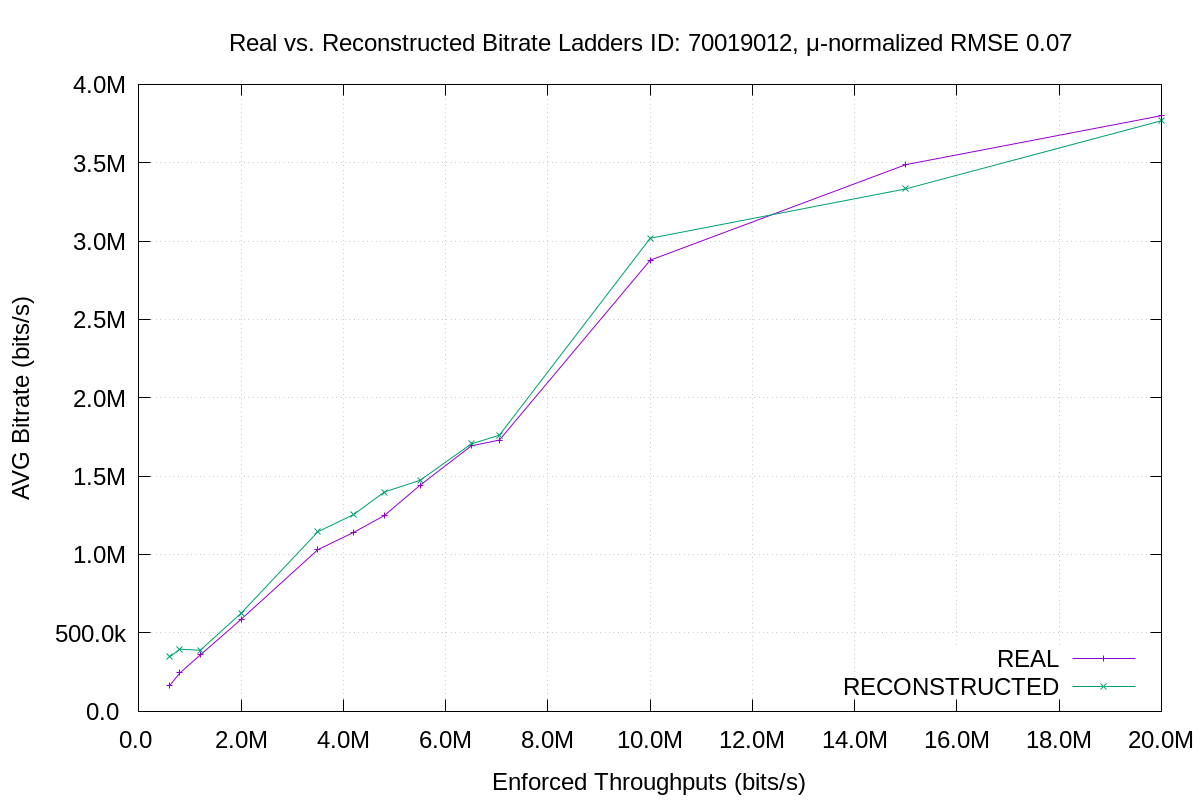
\includegraphics[width=\columnwidth]{img/70019012.png}
  \caption{Comparison between the HAR-based bitrate ladder (REAL) and the
  ADU-based reconstructed bitrate ladder for "Casino" ID: 70019012. Accuracy of
  reconstruction is shown as the RMSE.}
  \label{fig:bl_comparison_good}
\end{figure}

The plot above represents the "real" and reconstructed bitrate ladders.  The
accuracy of our prediction is represented by the RMSE, which is 0.07.  This
title's bitrate ladder gets reconstructed faithfully, and almost every title in
our database follow this trend. This is confirmed by further looking at the
average RMSE shown at the end of \Cref{tab:bitrate_ladders_stats}. Eventually,
63 titles have an RMSE less than 0.12, and 87 less than 0.16.
\Cref{fig:bl_comparison_good_1} and \Cref{fig:bl_comparison_good_2} are two
examples of reconstruction which RMSE is 0.12 and 0.16 respectively.

\newpage

\begin{figure}[!h]
  \centering
  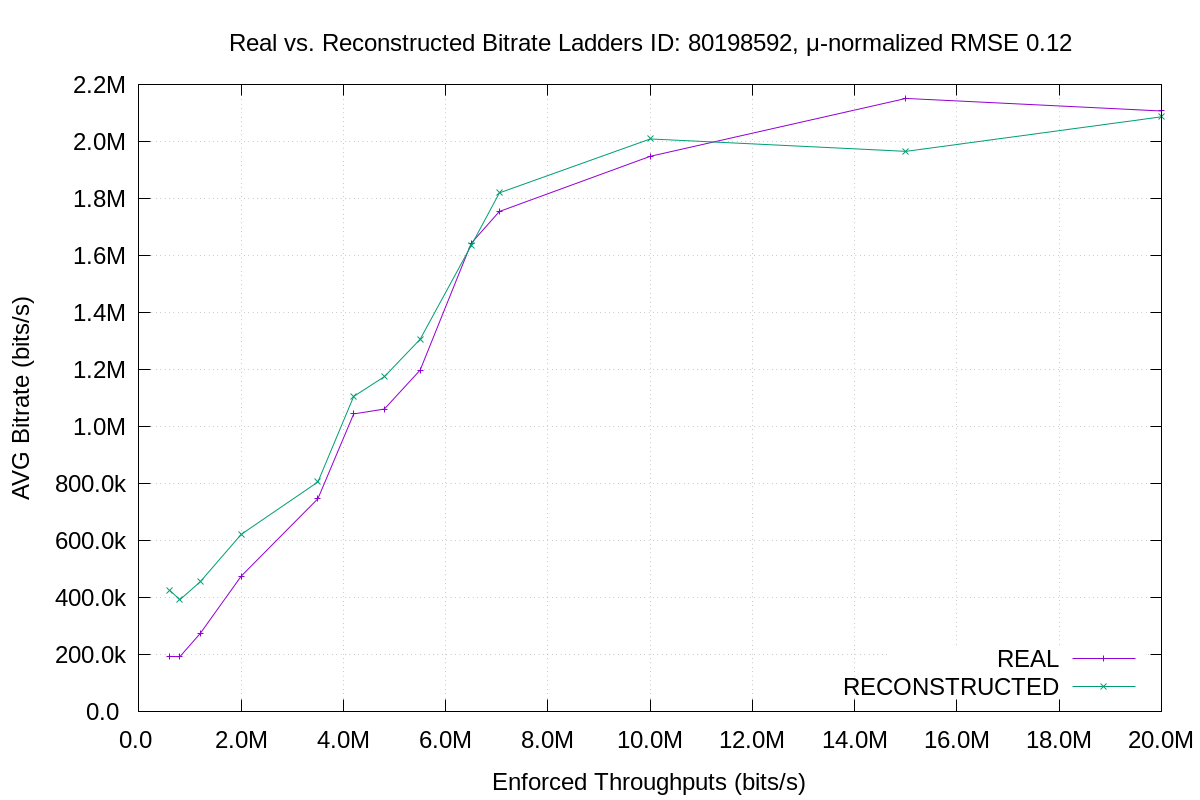
\includegraphics[width=\columnwidth]{img/80198592}
  \caption{Comparison between the HAR-based bitrate ladder (REAL) and the
  ADU-based reconstructed bitrate ladder for "Armed Response" ID: 80198592.
  Accuracy of reconstruction is shown as the RMSE.}
  \label{fig:bl_comparison_good_1}
\end{figure}

By looking at the above plot we spot two major areas where the differences
between the real and the reconstructed bitrates have greater impact on the
overall accuracy. Bottom left, when the enforced bandwidth and the bitrates are
low, and top right, at 15\emph{Mbps}. We focus our attention on the bottom-left
area, and notice how it correlates with the RMSE of the following plots.

\newpage
\begin{figure}[!h]
  \centering
  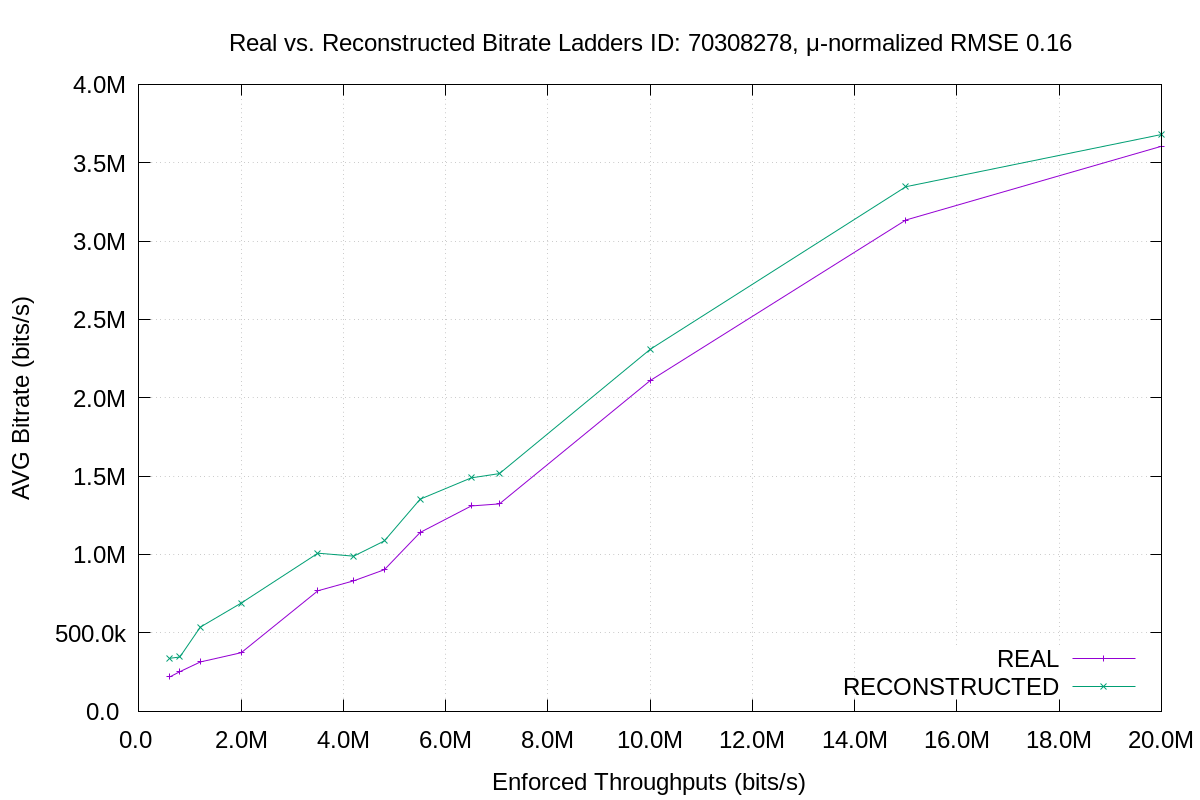
\includegraphics[width=\columnwidth]{img/70308278}
  \caption{Comparison between the HAR-based bitrate ladder (REAL) and the
  ADU-based reconstructed bitrate ladder for "Mission Blue" ID: 80198592.}
  \label{fig:bl_comparison_good_2}
\end{figure}

In this case we observe that with a greater RMSE, the two curves start to be
parallel to each other. By looking at the plot in \Cref{fig:bl_comparison_bad}
we see a magnified version of this behavior, and explain its existence.

\begin{figure}[!h]
  \centering
  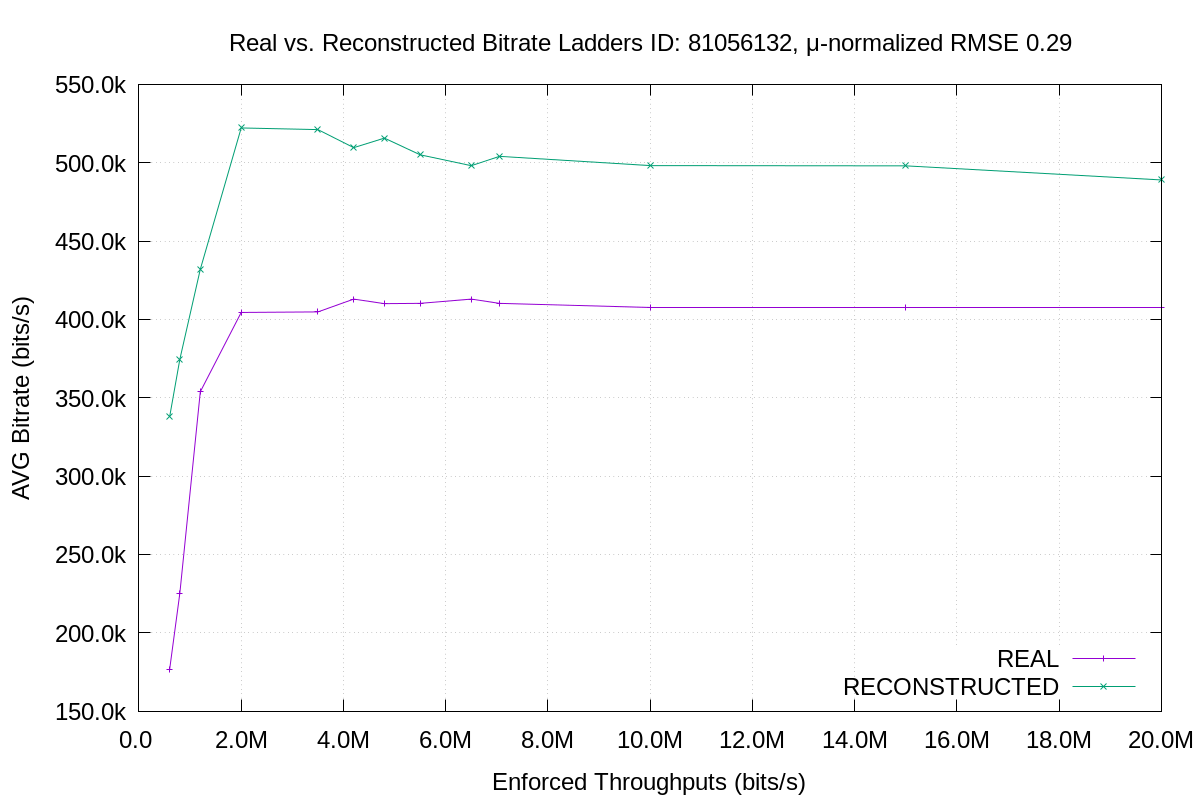
\includegraphics[width=\columnwidth]{img/81056132.png}
  \caption{Comparison between the HAR-based bitrate ladder (REAL) and the
  ADU-based reconstructed bitrate ladder for "Dirty John" ID: 81056132.}
  \label{fig:bl_comparison_bad}
\end{figure}

This plot represent a particular case of a

\todo{Finish this by explaining uniqueness of the bitrate ladders, arguing that
in a bigger DB we should try to cluster and complete the Video Identification
analysis, possibly making comparisons}

\chapter{Conclusions}\label{sec:conclusion}

We now analyze and discuss our system's strengths and weaknesses, arguing on
the conditions required to successfully perform the attack, and eventually,
present our perspective on possible future research.

\section{Contribution}

In \Cref{sec:results} we have given both quantitative and visual evidence of the
results achieved with our methodology. We now extend the analysis by abstracting
the context to a more realistic scenario. 

Throughout the description of our approach, we have ignore potential factors
that may be source of various types of errors when carrying out the attack in a
real scenario (\emph{e.g.} a public WLAN network). 

We have presented a revisited version of \cite{netflix-real-time} that, by
watching 4 minutes of video playback for a limited number of Netflix titles
(100), in stable network conditions, can faithfully reconstruct bitrate ladders
of movies encoded with an average bitrate greater than 1Mbps across 13
different enforced bandwidth levels. The 100 reconstructed bitrate ladders are
uniquely identifiable by their average bitrate, standard deviation, or median.

Our system identifies with approximately 86\% of accuracy the same set of
video titles across 8 \emph{unseen} bandwidth levels not previously captured in the
database. We have tested this behavior for several window sizes and conclude
that for majority of the titles, the average bitrate of, up to 20 subsequent
ADUs, represents a robust feature to reveal the content being streamed.

\subsection{Metrics}

\section{Benefits}

\todo{finish}

\section{Shortcomings and Feasibility}

\todo{finish}

The presence of various users in the network, for instance, may potentially
impact the quality of our resconstruction, especially if the content being
streamed is encoded at a low bitrate, or if the network bandwidth is unstable
(could cause the Netflix buffering algorithm to jump over different bitrate
levels during a 4 minute capture. 

\section{Future Work}

\todo{finish}

\chapter{Acknoweldgements}\label{sec:acknowledgements}

\emph{As I approach the conclusion of my studies at ETH Zurich, I would like to thank all the people that have helped me, in this awesome journey, my family, my close friends, and would like to express my gratitute to Prof. Dr. Ankit Singla and Phd student Melissa Licciardello, for their precious feedbacks and contribution to this work.}


\bibliographystyle{unsrtnat}
\bibliography{references.bib}

\begin{appendices}
    \crefalias{chapter}{appsec}
    \chapter{Bitrate Ladder Statistics}\label{app_ladder}

\begin{longtable}{|c|c c c|c c c|c|}
    \caption{Collected statistics for the bitrate ladders (values in
    \emph{Mbps})}\label{tab:bitrate_ladders_stats}\\
\hline
\textbf{Title ID} &
\multicolumn{3}{c|}{\textbf{Real}} &
\multicolumn{3}{c|}{\textbf{Reconstruced}} &
\multirow{2}{*}{\textbf{RMSE}} \\
& $\mu$ & $\sigma$ & $\tilde{y}$ & $\mu$ & $\sigma$ & $\tilde{y}$ & \\
\hline
\endhead
\hline
\endfoot
1151721 & 0.77 & 0.25 & 0.92 & 0.73 & 0.27 & 0.88 & 0.09 \\
14607635 & 0.81 & 0.25 & 0.95 & 0.74 & 0.27 & 0.89 & 0.12 \\
328438 & 0.88 & 0.34 & 1.06 & 0.89 & 0.37 & 1.06 & 0.06 \\
60000870 & 1.22 & 0.80 & 1.03 & 1.13 & 0.90 & 0.89 & 0.12 \\
60004481 & 0.75 & 0.19 & 0.85 & 0.65 & 0.19 & 0.76 & 0.16 \\
60020801 & 0.88 & 0.33 & 1.06 & 0.84 & 0.35 & 1.00 & 0.08 \\
60027695 & 0.93 & 0.38 & 1.13 & 0.92 & 0.41 & 1.08 & 0.06 \\
\rowcolor{lightgray}60033314 & 0.45 & 0.03 & 0.46 & 0.30 & 0.06 & 0.34 & 0.50 \\
70019012 & 1.59 & 1.09 & 1.40 & 1.52 & 1.15 & 1.25 & 0.07 \\
70021636 & 0.98 & 0.43 & 1.21 & 0.91 & 0.42 & 1.01 & 0.13 \\
70039177 & 0.66 & 0.16 & 0.74 & 0.58 & 0.21 & 0.66 & 0.18 \\
70041162 & 0.94 & 0.36 & 1.12 & 0.91 & 0.38 & 1.08 & 0.07 \\
70052701 & 1.40 & 1.10 & 1.07 & 1.30 & 1.18 & 0.95 & 0.10 \\
70084788 & 0.77 & 0.26 & 0.89 & 0.74 & 0.30 & 0.87 & 0.09 \\
70102778 & 0.73 & 0.23 & 0.87 & 0.71 & 0.26 & 0.85 & 0.08 \\
70103763 & 1.18 & 0.54 & 1.31 & 1.19 & 0.61 & 1.33 & 0.08 \\
70104894 & 0.82 & 0.28 & 0.96 & 0.78 & 0.31 & 0.92 & 0.09 \\
70112732 & 0.78 & 0.27 & 0.94 & 0.76 & 0.29 & 0.92 & 0.07 \\
70123542 & 0.86 & 0.31 & 1.03 & 0.81 & 0.33 & 0.94 & 0.10 \\
70123920 & 1.06 & 0.46 & 1.33 & 1.03 & 0.47 & 1.25 & 0.08 \\
70130445 & 0.68 & 0.10 & 0.70 & 0.60 & 0.12 & 0.68 & 0.15 \\
70167075 & 0.87 & 0.32 & 1.04 & 0.82 & 0.33 & 1.00 & 0.08 \\
70181730 & 1.80 & 1.65 & 1.51 & 1.75 & 1.59 & 1.44 & 0.09 \\
70208599 & 0.70 & 0.23 & 0.83 & 0.67 & 0.23 & 0.79 & 0.07 \\
\rowcolor{lightgray}70213513 & 0.66 & 0.12 & 0.70 & 0.51 & 0.14 & 0.59 & 0.29 \\
70216224 & 1.06 & 0.45 & 1.34 & 0.93 & 0.45 & 1.14 & 0.18 \\
70220028 & 0.83 & 0.17 & 0.90 & 0.69 & 0.18 & 0.80 & 0.21 \\
70243464 & 1.69 & 1.24 & 1.45 & 1.57 & 1.26 & 1.24 & 0.11 \\
70251894 & 0.79 & 0.25 & 0.93 & 0.76 & 0.30 & 0.92 & 0.10 \\
70264803 & 1.07 & 0.44 & 1.30 & 1.02 & 0.46 & 1.22 & 0.08 \\
70295915 & 0.48 & 0.08 & 0.51 & 0.44 & 0.10 & 0.49 & 0.13 \\
70296965 & 1.43 & 0.83 & 1.48 & 1.40 & 0.87 & 1.33 & 0.10 \\
70297757 & 0.63 & 0.18 & 0.72 & 0.61 & 0.19 & 0.72 & 0.07 \\
\rowcolor{lightgray}70298735 & 0.43 & 0.05 & 0.45 & 0.35 & 0.05 & 0.38 & 0.25 \\
\rowcolor{lightgray}70301367 & 0.44 & 0.05 & 0.46 & 0.33 & 0.07 & 0.36 & 0.35 \\
70305893 & 1.08 & 0.39 & 1.30 & 0.98 & 0.40 & 1.21 & 0.13 \\
70308278 & 1.44 & 1.03 & 1.09 & 1.25 & 1.04 & 0.90 & 0.16 \\
80000643 & 2.44 & 1.41 & 1.99 & 2.37 & 1.41 & 1.94 & 0.05 \\
80009431 & 1.64 & 1.10 & 1.43 & 1.56 & 1.17 & 1.27 & 0.10 \\
80013870 & 1.03 & 0.19 & 1.09 & 0.95 & 0.18 & 1.03 & 0.11 \\
80018689 & 1.05 & 0.44 & 1.24 & 1.00 & 0.46 & 1.16 & 0.08 \\
80023001 & 1.49 & 0.89 & 1.40 & 1.34 & 0.93 & 1.18 & 0.14 \\
80029196 & 1.12 & 0.32 & 1.30 & 0.98 & 0.31 & 1.16 & 0.15 \\
80031611 & 1.39 & 0.73 & 1.37 & 1.26 & 0.77 & 1.26 & 0.13 \\
80031715 & 1.01 & 0.44 & 1.17 & 0.99 & 0.44 & 1.19 & 0.06 \\
80033394 & 0.96 & 0.38 & 1.16 & 0.93 & 0.42 & 1.17 & 0.08 \\
80038359 & 0.84 & 0.31 & 0.99 & 0.82 & 0.32 & 0.96 & 0.06 \\
80052541 & 1.32 & 0.70 & 1.23 & 1.12 & 0.77 & 1.00 & 0.20 \\
80075563 & 1.40 & 0.65 & 1.26 & 1.24 & 0.72 & 1.04 & 0.16 \\
80081155 & 1.70 & 1.22 & 1.39 & 1.71 & 1.37 & 1.27 & 0.11 \\
80081770 & 1.13 & 0.44 & 1.35 & 1.00 & 0.49 & 1.22 & 0.15 \\
80091741 & 1.84 & 1.56 & 1.39 & 1.84 & 1.70 & 1.32 & 0.10 \\
80091879 & 1.08 & 0.48 & 1.34 & 1.02 & 0.49 & 1.28 & 0.08 \\
80093106 & 1.18 & 0.55 & 1.49 & 1.11 & 0.58 & 1.37 & 0.08 \\
80093138 & 1.68 & 1.21 & 1.49 & 1.60 & 1.26 & 1.31 & 0.11 \\
80096067 & 0.91 & 0.34 & 1.06 & 0.87 & 0.37 & 1.01 & 0.09 \\
\rowcolor{lightgray}80097391 & 0.50 & 0.04 & 0.51 & 0.40 & 0.04 & 0.41 & 0.25 \\
80102952 & 1.72 & 1.51 & 1.29 & 1.81 & 1.66 & 1.31 & 0.10 \\
80106307 & 1.52 & 0.76 & 1.59 & 1.47 & 0.78 & 1.54 & 0.05 \\
80109295 & 1.40 & 0.86 & 1.28 & 1.35 & 0.96 & 1.32 & 0.13 \\
80121387 & 1.60 & 0.84 & 1.52 & 1.54 & 0.89 & 1.38 & 0.07 \\
80121840 & 0.98 & 0.40 & 1.20 & 0.93 & 0.42 & 1.15 & 0.09 \\
80122759 & 1.46 & 0.79 & 1.57 & 1.32 & 0.82 & 1.34 & 0.14 \\
80128722 & 1.58 & 0.72 & 1.94 & 1.49 & 0.75 & 1.75 & 0.09 \\
80134721 & 1.96 & 1.05 & 2.16 & 1.88 & 1.08 & 2.00 & 0.06 \\
80135164 & 1.40 & 0.87 & 1.20 & 1.34 & 0.89 & 1.17 & 0.07 \\
\rowcolor{lightgray}80144140 & 0.52 & 0.10 & 0.56 & 0.42 & 0.11 & 0.48 & 0.23 \\
\rowcolor{lightgray}80163052 & 0.41 & 0.03 & 0.42 & 0.30 & 0.05 & 0.32 & 0.40 \\
80168188 & 2.07 & 1.37 & 1.74 & 2.02 & 1.49 & 1.65 & 0.07 \\
80169469 & 1.35 & 0.82 & 1.37 & 1.21 & 0.85 & 1.25 & 0.14 \\
80171659 & 2.06 & 1.68 & 1.59 & 1.96 & 1.72 & 1.35 & 0.09 \\
80174429 & 1.63 & 1.06 & 1.41 & 1.53 & 1.11 & 1.28 & 0.10 \\
80183328 & 1.22 & 0.59 & 1.16 & 1.07 & 0.60 & 0.96 & 0.15 \\
80184100 & 1.14 & 0.66 & 1.10 & 1.17 & 0.78 & 1.13 & 0.14 \\
80191608 & 1.28 & 0.59 & 1.51 & 1.22 & 0.63 & 1.42 & 0.08 \\
80192445 & 1.67 & 0.86 & 1.86 & 1.56 & 0.89 & 1.58 & 0.09 \\
80192815 & 1.32 & 0.68 & 1.19 & 1.27 & 0.72 & 1.20 & 0.07 \\
80195049 & 1.70 & 1.09 & 1.65 & 1.64 & 1.19 & 1.44 & 0.10 \\
80198592 & 1.21 & 0.62 & 1.17 & 1.14 & 0.70 & 1.06 & 0.12 \\
80199806 & 1.19 & 0.56 & 1.40 & 1.11 & 0.60 & 1.28 & 0.11 \\
80200961 & 0.99 & 0.50 & 0.88 & 0.91 & 0.56 & 0.77 & 0.13 \\
80202920 & 1.54 & 1.00 & 1.42 & 1.55 & 1.14 & 1.29 & 0.11 \\
80206300 & 0.82 & 0.28 & 0.94 & 0.79 & 0.31 & 0.95 & 0.09 \\
80210932 & 1.46 & 0.69 & 1.90 & 1.34 & 0.67 & 1.71 & 0.11 \\
80216541 & 1.61 & 0.79 & 1.77 & 1.51 & 0.83 & 1.57 & 0.09 \\
80217312 & 1.58 & 1.07 & 1.53 & 1.55 & 1.16 & 1.39 & 0.08 \\
80232502 & 1.21 & 0.64 & 1.10 & 1.11 & 0.70 & 1.00 & 0.10 \\
80239639 & 1.12 & 0.48 & 1.33 & 1.01 & 0.50 & 1.20 & 0.12 \\
80986885 & 1.38 & 0.79 & 1.45 & 1.38 & 0.84 & 1.47 & 0.05 \\
80991158 & 1.09 & 0.50 & 1.34 & 0.98 & 0.50 & 1.17 & 0.13 \\
80993095 & 0.96 & 0.43 & 1.01 & 0.89 & 0.48 & 0.96 & 0.11 \\
81000864 & 1.86 & 1.25 & 1.67 & 1.70 & 1.26 & 1.46 & 0.10 \\
81006261 & 1.34 & 0.85 & 1.21 & 1.37 & 0.94 & 1.21 & 0.08 \\
\rowcolor{lightgray}81056132 & 0.48 & 0.06 & 0.50 & 0.37 & 0.08 & 0.41 & 0.29 \\
81074663 & 1.67 & 1.01 & 1.70 & 1.63 & 1.10 & 1.57 & 0.08 \\
81075239 & 1.22 & 0.54 & 1.43 & 1.17 & 0.58 & 1.37 & 0.07 \\
81076251 & 1.21 & 0.61 & 1.12 & 1.08 & 0.66 & 0.98 & 0.14 \\
81080637 & 1.45 & 0.78 & 1.26 & 1.35 & 0.82 & 1.13 & 0.11 \\
81110498 & 2.35 & 1.33 & 2.08 & 2.22 & 1.50 & 2.04 & 0.20 \\
896970 & 1.55 & 0.96 & 1.37 & 1.39 & 0.99 & 1.15 & 0.13 \\
\hline
\multicolumn{7}{|l}{\textbf{AVERAGE}} & 0.12 \\
\end{longtable}

\end{appendices}

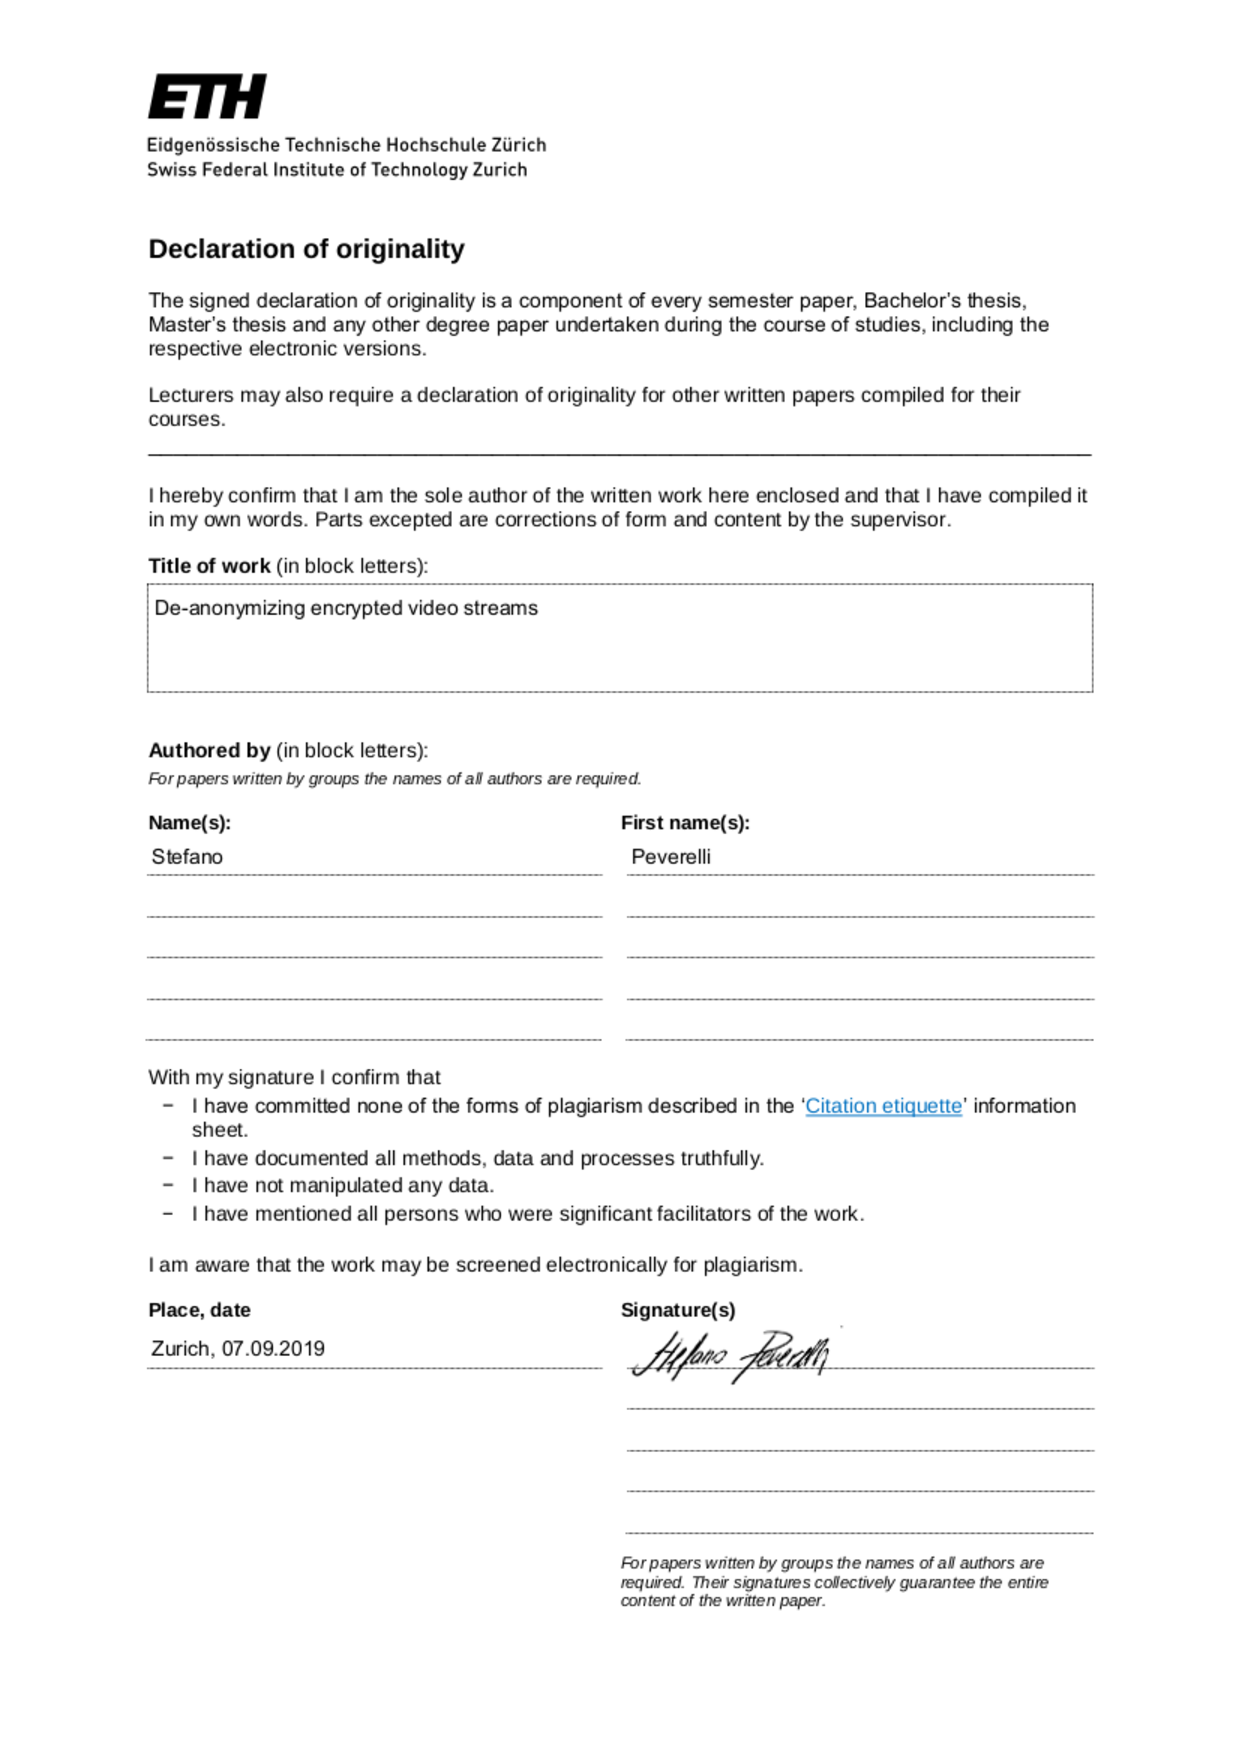
\includepdf[pages=-]{declaration_of_originality.pdf}

\end{document}
